\subsection{Minkowski 不等式}

设 X 是一个局部紧空间，\(\mu\) 是 X 上的一个测度。在定义于 X 上的正数值函数（有限或非有限）所成的集中，函数 \(|\mu|^{*}(f)\) 是正的、正齐次的、递增的且凸的（ \(\S1\) , No.~3, 命题 10、11 与 12）。

命题 1. --- 对每个实数 \(p \geqslant 1\) 与每对正函数 \(f, g\) （有限或非有限，定义于 \(X\) 上），

\[
\left(| \mu | ^ {*} ((f + g) ^ {p})\right) ^ {1 / p} \leqslant \left(| \mu | ^ {*} (f ^ {p})\right) ^ {1 / p} + \left(| \mu | ^ {*} (g ^ {p})\right) ^ {1 / p}\tag{1}
\]

（Minkowski 不等式）。

当右端的项之一等于 \(+\infty\) 时，不等式 (1) 是明显的。在相反的情形，\(f\) 与 \(g\) 几乎处处有限（§2, No.~3, 命题 7）。若 \(f_1\) 与 \(g_1\) 是分别等价于 \(f\) 与 \(g\) 的有限正函数，则 \(f_1^p\) 、 \(g_1^p\) 与 \((f_1 + g_1)^p\) 分别等价于 \(f^p\) 、 \(g^p\) 与 \((f + g)^p\) ，而由于等价的正函数具有相同的上积分（§2, No.~3, 命题 6），我们只需就 \(f\) 与 \(g\) 处处有限的情形证明不等式 (1) ；但在这一情形，该不等式是 Ch. I, No.~2 的命题 3 中证明的一般 Minkowski 不等式的特例。

我们还将有机会用到下述初等不等式：若 \(p \geqslant 1\) ，则对任意数 \(a \geqslant 0\) 、 \(b \geqslant 0\) ，

\[
a ^ {p} + b ^ {p} \leqslant (a + b) ^ {p}.\tag{2}
\]

若 \(a = b = 0\) ，或数 \(a, b\) 之一等于 \(+\infty\) ，则不等式是明显的；若 \(a, b\) 有限且 \(a + b > 0\) ，则它可写成

\[
\left(\frac {a}{a + b}\right) ^ {p} + \left(\frac {b}{a + b}\right) ^ {p} \leqslant 1,
\]

这由以下事实得出：

\[
\left(\frac {a}{a + b}\right) ^ {p} \leqslant \frac {a}{a + b}, \quad \left(\frac {b}{a + b}\right) ^ {p} \leqslant \frac {b}{a + b} \quad \text { and } \quad \frac {a}{a + b} + \frac {b}{a + b} = 1.
\]

\subsection{\texorpdfstring{半范数 \(\mathbf{N}_p\)}{半范数 N sub p}}

在以下全部内容中，F 表示域 R 或域 C 上的一个完备赋范向量空间（即 Banach 空间）；元素 \(z \in F\) 的范数将记作 \(|z|\) 。给定集合 A 到 F 中的一个映射 f，我们用 \(|f|\) 表示映射 \(x \mapsto |\mathbf{f}(x)|\) ，即 A 到 \(R_{+}\) 中的一个映射（必须注意 \(|f|\) 是一个数值函数，而不是一个数）。

定义 1. --- 设 X 是一个局部紧空间，\(\mu\) 是 X 上的一个测度。对 X 到 Banach 空间 F 中的每个映射 f，以及对每个使 \(1 \leqslant p < +\infty\) 的数 p，我们用 \(\mathrm{N}_p(\mathbf{f}, \mu)\) （或简作 \(\mathrm{N}_p(\mathbf{f})\) ）表示正数 \((\int^* |\mathbf{f}|^p d|\mu|)^{1/p}\) 。

注意，数 \(N_{p}(\mathbf{f})\) 可以等于 \(+\infty\) 。

命题 2. --- 若 f 与 g 是 X 到 F 中的两个映射，且 \(\alpha\) 是任一标量 \(\neq 0\) ，则对 \(1 \leqslant p < +\infty\) ，

\begin{enumerate}
\def\labelenumi{(\arabic{enumi})}
\setcounter{enumi}{2}
\tightlist
\item
\end{enumerate}

\[
\mathrm{N} _ {p} (\alpha \mathbf {f}) = | \alpha | \mathrm{N} _ {p} (\mathbf {f})\tag{4}
\]

\[
\mathrm{N} _ {p} (\mathbf {f} + \mathbf {g}) \leqslant \mathrm{N} _ {p} (\mathbf {f}) + \mathrm{N} _ {p} (\mathbf {g}).
\]

因为，关系式 (3) 由定义 1 以及 \(|\mu|^*\) 是正齐次的这一事实立得；另一方面，由于 \(|\mathbf{f} + \mathbf{g}| \leqslant |\mathbf{f}| + |\mathbf{g}|\) ，不等式 (4) 由 Minkowski 不等式 (1) 以及 \(|\mu|^*\) 是递增的这一事实得出。

我们把定义 1 推广到定义在 X 上的数值函数（有限或非有限）的情形，仍令

\[
\mathrm{N} _ {p} (f) = \left(\int^ {*} | f | ^ {p} d | \mu |\right) ^ {1 / p}
\]

对这样的函数 \(f\) 。立即可见，当 \(f + g\) 在 \(X\) 上有定义且 \(\alpha \neq 0\) 时，关系式 (3) 与 (4) 对这些函数也成立。此外：

定理 1（可数凸性定理）. --- 设 \((f_n)\) 是定义在 X 上的函数 \(\geqslant 0\) （有限或非有限）的一个序列。对 \(1 \leqslant p < +\infty\) ，

\[
\mathrm{N} _ {p} \left(\sum_ {n = 1} ^ {\infty} f _ {n}\right) \leqslant \sum_ {n = 1} ^ {\infty} \mathrm{N} _ {p} (f _ {n}).\tag{5}
\]

令 \(f = \sum_{n=1}^{\infty} f_n\) ；\(f\) 是递增函数序列 \(g_n = \sum_{k=1}^{n} f_k\) 的上包络；\(N sub p(f)\) 的定义以及 §1, No.~3 的定理 3 表明 \(\mathrm{N}_{p}(f)=\sup_{n}\mathrm{N}_{p}(g_{n})\) 。但由命题 1 有 \(\mathrm{N}_{p}(g_{n})\leqslant\sum_{k=1}^{n}\mathrm{N}_{p}(f_{k})\) ，由此得不等式 (5)。

命题 3. --- 若 \(\mathbf{f}\) 与 \(\mathbf{g}\) 是 X 到 Banach 空间 F 中的两个等价映射，则 \(\mathrm{N}_p(\mathbf{f} - \mathbf{g}) = 0\) 对 \(1 \leqslant p < +\infty\) 成立；反之，若 \(\mathrm{N}_p(\mathbf{f} - \mathbf{g}) = 0\) 对某个值 \(p \geqslant 1\) 成立，则 \(\mathbf{f}\) 与 \(\mathbf{g}\) 等价。命题由 §2, No.~3 的定理 1 立得。

若 \(\mathbf{f}\) 与 \(\mathbf{g}\) 是 \(X\) 到 \(F\) 中的两个等价映射，则 \(\mathrm{N}_p(\mathbf{f}) = \mathrm{N}_p(\mathbf{g})\) 对一切 \(p \geqslant 1\) 成立（ \(\S 2\) , No.~3, 命题 6）；于是 \(\mathrm{N}_p(\mathbf{f})\) 只依赖于类 \(\widetilde{\mathbf{f}}\) （\(\mathbf{f}\) 的），且依定义令 \(\mathrm{N}_p(\widetilde{\mathbf{f}}) = \mathrm{N}_p(\mathbf{f})\) 。由于 \(X\) 到 \(F\) 中的映射的类构成一个向量空间（ \(\S 2\) , No.~4），关系式 (3) 与 (4) 也可写成

\begin{enumerate}
\def\labelenumi{(\arabic{enumi})}
\setcounter{enumi}{5}
\tightlist
\item
\end{enumerate}

\[
\mathrm{N} _ {p} (\alpha \widetilde {\mathbf {f}}) = | \alpha | \mathrm{N} _ {p} (\widetilde {\mathbf {f}})\tag{7}
\]

\[
\mathrm{N} _ {p} (\widetilde {\mathbf {f}} + \widetilde {\mathbf {g}}) \leqslant \mathrm{N} _ {p} (\widetilde {\mathbf {f}}) + \mathrm{N} _ {p} (\widetilde {\mathbf {g}}).
\]

类似地，对等价数值函数（有限或非有限）的每个类，定义 \(\mathrm{N}_{p}(\tilde{\mathbf{f}})\) 。

于是，可对下述函数定义 \(\mathrm{N}_{p}(\mathbf{f})\) ：该函数在 X 上几乎处处有定义，取值于 F （相应地 \(\overline{R}\) ）中，方法是令 \(\mathrm{N}_{p}(\mathbf{f})=\mathrm{N}_{p}(\widetilde{\mathbf{f}})\) ；此时显然关系式 (3) 与 (4) 仍成立（在数值函数（有限或非有限）的情形，假定 \(\alpha\neq0\) 且 \(f+g\) 几乎处处有定义）。

若 \(0 < p < 1\) ，仍令 \(\mathrm{N}_p(\mathbf{f}) = (\int^* |\mathbf{f}|^p d|\mu|)^{1/p}\) ，但不等式 (4) 与 (5) 不再成立（参见 Ch. I, 习题 6 与 Ch. IV, §6, 习题 13）。

\subsection{\texorpdfstring{空间 \(\mathcal{F}_{\mathrm{F}}^{p}\)}{空间 F sub F to the p}}

设 F 是一个 Banach 空间，\(\mathcal{F}(X;F)\) （或简作 \(F_{F}\) ）是 X 到 F 中所有映射所成的向量空间。对 \(1 \leqslant p < +\infty\) ，我们将用 \(\mathcal{F}^{p}(X,\mu;F)\) 或 \(\mathcal{F}_{\mathrm{F}}^{p}(X,\mu)\) ，或简作 \(\mathcal{F}_{\mathrm{F}}^{p}(\mu)\) ，或 \(\mathcal{F}_{\mathrm{F}}^{p}\) （若不致引起混淆），表示 X 到 F 中使 \(N_{p}(\mathbf{f}) < +\infty\) 的映射 f 所成之集（我们用 \(F^{p}\) 代替 \(F_{R}^{p}\) ）。显然 \(\mathcal{F}_{\mathrm{F}}^{p}(|\mu|) = \mathcal{F}_{\mathrm{F}}^{p}(\mu)\) 。由 No.~2 的命题 2 立得：\(F_{F}^{p}\) 是 \(F_{F}\) 的一个线性子空间，且 \(N_{p}(\mathbf{f})\) 是这个空间上的一个半范数。我们总假定（除明确声明相反情形外）\(F_{F}^{p}\) 赋有由这个半范数定义的拓扑；我们称这拓扑为 p 阶平均收敛拓扑（对 p = 1，简称平均收敛拓扑；对 p = 2，也称«均方收敛拓扑»）。我们称 \(F_{F}^{p}\) 上关于这拓扑收敛于 f 的滤子 G （相应地，序列 \((\mathbf{f}_{n})\) ，其元素属于 \(F_{F}^{p}\) ）为 p 阶平均收敛于 f 的；这就是说，\(N_{p}(\mathbf{g}-\mathbf{f})\) 关于 G 趋于 0 （相应地， \(N_{p}(\mathbf{f}_{n}-\mathbf{f})\) 当 n 趋于无穷时趋于 0）。

这一术语可直接推广到下述情形：函数 \(f_{n}\) 与函数 f 只是几乎处处有定义（或取值于 \(\overline{R}\) ，且几乎处处有定义并有限）。

注意，局部凸空间 \(F_{F}^{p}\) 一般不是 Hausdorff 的；0 在这个空间中的闭包是 X 到 F 中的可忽略映射所成的线性子空间 \(N_{F}\) （No.~2, 命题 3）。

注. --- 设 F 是复数域 C 上的一个 Banach 空间；于是，对每个函数 \(f \in F_{F}^{p}\) 与每个复数 \(\alpha\) ，\(\alpha f\) 属于 \(F_{F}^{p}\) 且 \(N_{p}(\alpha f) = |\alpha| N_{p}(f)\) ；换句话说，\(F_{F}^{p}\) 也是 C 上的一个向量空间，且 \(N_{p}(f)\) 是这个复向量空间上的一个半范数（TVS, II, §1）。

命题 4. --- 设 B 是 \(F_{F}^{p}\) 上的一个滤子基。假定存在紧集 \(K \subset X\) ，使对每个集 \(M \in B\) ，所有映射 \(f \in M\) 的支集都含于 K。在这些条件下，若 B 在 X 上一致收敛于 \(f_{0}\) ，则 \(f_{0}\) 属于 \(F_{F}^{p}\) 且 B p 阶平均收敛于 \(f_{0}\) 。

这等价于说：在支集含于一个固定紧集的映射 \(f \in F_{F}^{p}\) 所成之集上，一致收敛拓扑细于 p 阶平均收敛拓扑。

因为，设 \(h\) 是 \(X\) 到 \([0,1]\) 中的一个连续映射，具有紧支集，且在 \(K\) 上等于 1（Ch. III, §1, No.~2, 引理 1）。对每个 \(\varepsilon > 0\) ，存在 \(M \in \mathfrak{B}\) ，使对每个映射 \(\mathbf{f} \in M\) ，有 \(|\mathbf{f}(x) - \mathbf{f}_0(x)| \leqslant \varepsilon h(x)\) 对所有 \(x \in X\) 成立。由此得出 \(N sub p(\mathbf{f} - \mathbf{f}_0) \leqslant \varepsilon N sub p(h)\) ，命题得证。

命题 5. --- 局部凸空间 \(\mathcal{F}_{\mathrm{F}}^{p}\) 是完备的。

由于与 \(\mathcal{F}_{\mathrm{F}}^{p}\) 相伴的 Hausdorff 空间是一个赋范空间，只需证明每个 Cauchy 序列 \((\mathbf{f}_n)\) （\(\mathcal{F}_{\mathrm{F}}^{p}\) 中的）对于 \(p\) 阶平均收敛拓扑都有一个极限（GT, IX, §2, No.~6, 命题 9）。按假设，对每个 \(\varepsilon > 0\) 存在整数 \(m_0\) ，使关系 \(m \geqslant m_0\) 、 \(n \geqslant m_0\) 蕴涵 \(\mathrm{N}_p(\mathbf{f}_n - \mathbf{f}_m) \leqslant \varepsilon\) 。于是可以对 \(k\) 用归纳法定义一个严格递增的整数序列 \((n_k)\) （ \(\geqslant 0\) ），使 \(\mathrm{N}_p(\mathbf{f}_{n_{k+1}} - \mathbf{f}_{n_k}) \leqslant 2^{-k}\) 。若我们能证明通项为 \(\mathbf{g}_k = \mathbf{f}_{n_{k+1}} - \mathbf{f}_{n_k}\) （ \(k \geqslant 1\) ）的级数 \(p\) 阶平均收敛，则它将有和 \(\mathbf{g} \in \mathcal{F}_{\mathrm{F}}^p\) ，而 \(\mathbf{f} = \mathbf{g} + \mathbf{f}_{n_1}\) 将是序列 \((\mathbf{f}_{n_k})\) 在 \(\mathcal{F}_{\mathrm{F}}^p\) 中的极限；于是 \(\mathbf{f}\) 是序列 \((\mathbf{f}_n)\) 的一个接触点；由于这个序列是 Cauchy 序列，它将以 f 为极限，从而命题 5 得证（GT, II, §3, No.~2, 命题 5 的推论 2）。

于是命题 5 是下述命题的推论：

命题 6. --- 设 \((\mathbf{f}_{n})\) 是 \(F_{F}^{p}\) 中函数的一个序列，使 \(\sum_{n=1}^{\infty}\mathrm{N}_{p}(\mathbf{f}_{n})<+\infty\) 。在这些条件下，通项为 \(\mathbf{f}_{n}(x)\in\mathbf{F}\) 的级数在 X 上几乎处处绝对收敛。在级数收敛的点处令 \(\mathbf{f}(x)=\sum_{n=1}^{\infty}\mathbf{f}_{n}(x)\) ，在别处令 \(\mathbf{f}(x)=0\) ，则函数 f 属于 \(F_{F}^{p}\) 且是通项为 \(f_{n}\) 的级数的和（对于 p 阶平均收敛拓扑）；更精确地说，对每个 \(n\geqslant0\) ，

\[
\mathrm{N} _ {p} \left(\mathbf {f} - \sum_ {k = 1} ^ {n} \mathbf {f} _ {k}\right) \leqslant \sum_ {k = n + 1} ^ {\infty} \mathrm{N} _ {p} (\mathbf {f} _ {k}).\tag{8}
\]

考虑正函数（有限或非有限） \(g(x) = \sum_{n=1}^{\infty} |\mathbf{f}_n(x)|\) 。由可数凸性定理（No.~2, 定理 1），

\[
\mathrm{N} _ {p} (g) \leqslant \sum_ {n = 1} ^ {\infty} \mathrm{N} _ {p} (\mathbf {f} _ {n}) <   + \infty ;
\]

于是 \(g\) 几乎处处有限（§2, No.~3, 命题 7），这表明通项为 \(\mathbf{f}_n(x)\) 的级数几乎处处绝对收敛。由于 \(F\) 是完备的，这级数几乎处处收敛，且对每个 \(x \in X\) ，有 \(|\mathbf{f}(x)| \leqslant \sum_{n=1}^{\infty} |\mathbf{f}_n(x)| = g(x)\) ，由此得

\[
\mathrm{N} _ {p} (\mathbf {f}) \leqslant \mathrm{N} _ {p} (g) \leqslant \sum_ {n = 1} ^ {\infty} \mathrm{N} _ {p} (\mathbf {f} _ {n}) <   + \infty ,
\]

这就证明了 \(\mathbf{f}\) 属于 \(\mathcal{F}_{\mathrm{F}}^{p}\) 。另一方面，对每个整数 \(n\) ，

\[
\left| \mathbf {f} (x) - \sum_ {k = 1} ^ {n} \mathbf {f} _ {k} (x) \right| \leqslant \sum_ {k = n + 1} ^ {\infty} | \mathbf {f} _ {k} (x) |
\]

几乎处处成立，由此得 \(\mathrm{N}_{p}\left(\mathbf{f}-\sum_{k=1}^{n}\mathbf{f}_{k}\right)\leqslant\sum_{k=n+1}^{\infty}\mathrm{N}_{p}(\mathbf{f}_{k})\) 。按假设，通项为 \(\mathrm{N}_{p}(\mathbf{f}_{n})\) 的级数收敛；因此，对每个 \(\varepsilon > 0\) ，存在整数 \(n\) 使 \(\sum_{k=n+1}^{\infty} \mathrm{N}_{p}(\mathbf{f}_{k}) \leqslant \varepsilon\) ，而不等式 (8) 证明了 \(\mathbf{f}\) 是通项为 \(\mathbf{f}_{n}\) 的级数的和（对于 \(p\) 阶平均收敛拓扑）。

于是命题 5 与命题 6 完全得证。

\subsection{\texorpdfstring{\(p\) 次幂可积函数}{p 次幂可积函数}}

向量空间 \(\mathcal{K}(X;F)\) （若不致引起混淆，我们简记作 \(K_{F}\) ）由 X 到 F 中的具有紧支集的连续函数组成，它显然是每个向量空间 \(F_{F}^{p}\) 的子空间。

定义 2. --- 给定一个局部紧空间 X、X 上的一个测度 \(\mu\) 与一个 Banach 空间 F，我们用 \(\mathcal{L}_{\mathrm{F}}^{p}(\mathrm{X},\mu)\) （或简作 \(\mathcal{L}_{\mathrm{F}}^{p}(\mu)\) ，或 \(\mathcal{L}_{\mathrm{F}}^{p}\) ）表示局部凸空间 \(\mathcal{F}_{\mathrm{F}}^{p}(\mathrm{X},\mu)\) 中由 X 到 F 中的具有紧支集的连续映射所成的向量空间 \(\mathcal{K}(\mathrm{X};\mathrm{F})\) 的闭包。我们用 \(\mathrm{L}_{\mathrm{F}}^{p}(\mathrm{X},\mu)\) （或 \(\mathrm{L}_{\mathrm{F}}^{p}(\mu)\) ，或 \(\mathrm{L}_{\mathrm{F}}^{p}\) ）表示与 \(\mathcal{L}_{\mathrm{F}}^{p}(\mathrm{X},\mu)\) 相伴的（赋范）Hausdorff 空间。属于 \(\mathcal{L}_{\mathrm{F}}^{p}\) 的函数称为 \(p\) 次幂可积函数（*）。

显然 \(\mathcal{L}_{\mathrm{F}}^{p}(\mathrm{X},|\mu |) = \mathcal{L}_{\mathrm{F}}^{p}(\mathrm{X},\mu)\) 且 \(\mathrm{L}_{\mathrm{F}}^{p}(\mathrm{X},|\mu |) = \mathrm{L}_{\mathrm{F}}^{p}(\mathrm{X},\mu)\) 。

我们将用 \(L^{p}\) 与 \(L^{p}\) 代替 \(L_{R}^{p}\) 与 \(L_{R}^{p}\) （当这不致引起混淆时，或用 \(L_{C}^{p}\) 与 \(L_{C}^{p}\) 代替）。若 F 是一个复 Banach 空间，则 \(L_{F}^{p}\) 与 \(L_{F}^{p}\) 赋有域 C 上的拓扑向量空间结构（No.~3, 注）。

显然，\(F_{F}^{p}\) 中每个与 \(L_{F}^{p}\) 中一个函数等价的函数都属于 \(L_{F}^{p}\) 。取值于 F 且在 X 上几乎处处有定义的函数，若它与 \(L_{F}^{p}\) 中的一个函数等价，也称为 p 次幂可积的；类似地，取值于 \(\overline{R}\) 、在 X 上几乎处处有定义且有限的函数，若它与 \(L^{p}\) 中的一个函数等价，就称为 p 次幂可积的。

于是，\(L_{F}^{p}\) （相应地 \(L^{p}\) ）中的函数就是在整个 X 上有定义（相应地，在整个 X 上有定义且有限）的 p 次幂可积函数。在本节及下一节中，对 \(L_{F}^{p}\) （相应地 \(L^{p}\) ）中的函数证明的大多数命题，都可以立即推广到并非处处有定义（相应地，并非处处有定义且有限）的 p 次幂可积函数；我们通常把陈述并证明这些结果的任务留给读者。

注记. --- 1) 如已指出的（§2, No.~5），取值于 F 的 p 次幂可积函数一般不构成向量空间。

\begin{enumerate}
\def\labelenumi{\arabic{enumi})}
\setcounter{enumi}{1}
\tightlist
\item
  一般地，空间 \(\mathcal{F}_{\mathrm{F}}^{p}\) 不同于其子空间 \(\mathcal{L}_{\mathrm{F}}^{p}\) （§4, 习题 8）。
\end{enumerate}

定义 2 立即给出下述判别法：

命题 7. --- 为使函数 f 属于 \(L_{F}^{p}\) ，必须且只须对每个 \(\varepsilon > 0\) ，存在具有紧支集的连续函数 g 使 \(\mathrm{N}_{p}(\mathbf{f} - \mathbf{g}) \leqslant \varepsilon\) 。

换句话说，\(L_{F}^{p}\) 中的函数是具有紧支集的连续函数序列（对于 p 阶平均收敛拓扑）的极限。

命题 8. --- 设 f 是几乎处处有定义的数值函数（有限或非有限）；若对每个 \(\varepsilon > 0\) ，存在两个 p 次幂可积函数 g、h ，使 \(g \leqslant f \leqslant h\) 几乎处处成立且 \(\mathrm{N}_{p}(h - g) \leqslant \varepsilon\) ，则 f 是 p 次幂可积的。

因为，\(f\) 几乎处处有限且 \(\mathrm{N}_p(f - g) \leqslant \mathrm{N}_p(h - g) \leqslant \varepsilon\) ；于是命题 7 表明 \(f\) 是 \(p\) 次幂可积的。

由于按定义 \(L_{F}^{p}\) 是 \(F_{F}^{p}\) 的一个闭子空间，且后一空间是完备的（No.~3, 命题 5），我们有下述结果（GT, II, §3, No.~4, 命题 8）：

定理 2. --- 空间 \(\mathcal{L}_{\mathrm{F}}^{p}\) 是完备的；空间 \(\mathrm{L}_{\mathrm{F}}^{p}\) 是一个 Banach 空间。

在空间 \(L_{F}^{p}\) 中，一个类的范数 \(\mathrm{N}_{p}(\widetilde{\mathbf{f}})\) 也记作 \(\| \widetilde{f} \|_{p}\) 。

定理 2 可以加强如下：

定理 3. --- 设 \((\mathbf{f}_n)\) 是空间 \(\mathcal{L}_{\mathrm{F}}^p\) 中的一个 Cauchy 序列；存在一个子序列 \((\mathbf{f}_{n_k})\) （\((\mathbf{f}_n)\) 的），它具有下列性质：

\(1^{\circ}\) 通项为 \(\mathrm{N}_p(\mathbf{f}_{n_{k + 1}} - \mathbf{f}_{n_k})\) 的级数收敛；

\(2^{\circ}\) 通项为 \(\mathbf{f}_{n_{k+1}}(x) - \mathbf{f}_{n_k}(x)\) 的级数几乎处处绝对收敛；

\(3^{\circ}\) 若 \(\mathbf{f}\) 是定义在 X 上且几乎处处等于序列 \((\mathbf{f}_{n_k}(x))\) 的极限的函数，则 \(\mathbf{f}\) 属于 \(\mathcal{L}_{\mathrm{F}}^p\) 且序列 \((\mathbf{f}_n)\) \(p\) 阶平均收敛于 \(\mathbf{f}\) ；

\(4^{\circ}\) 存在下半连续函数 \(g \geqslant 0\) 使 \(\mathrm{N}_p(g) < +\infty\) ，且对每个 \(k\) ，有 \(|\mathbf{f}_{n_k}(x)| \leqslant g(x)\) 对所有 \(x \in X\) 成立。

如同 No.~3 命题 5 的证明中那样，只需用归纳法定义序列 \((n_k)\) ，使 \(\mathrm{N}_p(\mathbf{f}_{n_{k+1}} - \mathbf{f}_{n_k}) \leqslant 2^{-k}\) ；于是 \(2^\circ\) 与 \(3^\circ\) 由 No.~3 的命题 6 以及 \(\mathcal{L}_{\mathrm{F}}^p\) 在 \(\mathcal{F}_{\mathrm{F}}^p\) 中为闭这一事实得出。另一方面，若 \(h(x)\) 是通项为 \(|\mathbf{f}_{n_{k+1}}(x) - \mathbf{f}_{n_k}(x)|\) 的级数的和，则 No.~2 的定理 1 表明 \(\mathrm{N}_p(h) < +\infty\) ；因此，由 \(|\mu|^*\) 的定义，存在下半连续函数 \(g \geqslant h + |\mathbf{f}_{n_1}|\) 使 \(\mathrm{N}_p(g) < +\infty\) ，证明遂告完成。

推论 1. --- 若 Cauchy 序列 \((\mathbf{f}_{n})\) （空间 \(L_{F}^{p}\) 中的）使序列 \((\mathbf{f}_{n}(x))\) 几乎处处收敛于 \(\mathbf{f}(x)\) ，则 f 是 p 次幂可积的，且序列 \((\mathbf{f}_{n})\) p 阶平均收敛于 f。

因为，存在子序列 \((\mathbf{f}_{n_{k}})\) （\((\mathbf{f}_{n})\) 的），使 \((\mathbf{f}_{n_{k}}(x))\) 几乎处处收敛于 \(\mathbf{g}(x)\) ，其中 g 是 \(L_{F}^{p}\) 中的一个函数，使 \((\mathbf{f}_{n})\) p 阶平均收敛于 g。于是假设蕴涵 \(\mathbf{f}(x)=\mathbf{g}(x)\) 几乎处处成立，推论得证。

推论 2. --- 设 E 是 \(L_{F}^{p}\) 的一个稠密子集。对每个函数 \(f \in L_{F}^{p}\) ，存在 E 中函数的一个序列 \((\mathbf{g}_{n})\) ，它具有下列性质：

\(1^{\circ}\) 序列 \((\mathbf{g}_n)\) \(p\) 阶平均收敛于 \(\mathbf{f}\) ；

\(2^{\circ}\) 对几乎每个 \(x \in \mathbf{X}\) ，序列 \((\mathbf{g}_n(x))\) 收敛于 \(\mathbf{f}(x)\) 。

因为，由于空间 \(L_{F}^{p}\) 是可度量的，存在一个 Cauchy 序列 \((\mathbf{f}_{n})\) （\(L_{F}^{p}\) 中的），由 E 中的函数组成且 p 阶平均收敛于 f（GT, IX, §2, No.~6, 命题 8）；只需对这个序列应用定理 3。

推论 2 特别适用于取 E 为具有紧支集的连续函数所成的空间 \(K_{F}\) 的情形。

\pandocbounded{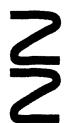
\includegraphics[keepaspectratio]{images/part001_fce77adb.jpg}}

注记. --- 1) Cauchy 序列 \((\mathbf{f}_n)\) （\(\mathcal{L}_{\mathrm{F}}^{p}\) 中的）可以使序列 \((\mathbf{f}_n(x))\) 在 X 的任何点都不收敛（习题 1）。

\begin{enumerate}
\def\labelenumi{\arabic{enumi})}
\setcounter{enumi}{1}
\tightlist
\item
  若 \(\mathbf{f}\) 属于 \(\mathcal{L}_{\mathrm{F}}^{p}\) ，并不总能找到具有紧支集的连续函数的序列 \((\mathbf{f}_n)\) ，使序列 \((\mathbf{f}_n(x))\) 在 \(X\) 上处处收敛于一个几乎处处等于 \(\mathbf{f}(x)\) 的函数（§4, 习题 4 c)）。
\end{enumerate}

\subsection{p 次幂可积函数的性质}

定理 4. --- 设 F 与 G 是两个 Banach 空间，u 是 F 到 G 中的一个连续线性映射。对每个函数 \(f \in L_{F}^{p}\) ，复合函数 \(u \circ f\) 属于 \(L_{G}^{p}\) 。

设 \(\mathbf{f} \in \mathcal{L}_{\mathrm{F}}^{p}\) ；对每个 \(\varepsilon > 0\) ，存在函数 \(\mathbf{g} \in \mathcal{K}_{\mathrm{F}}\) 使 \(\mathrm{N}_p(\mathbf{f} - \mathbf{g}) \leqslant \varepsilon\) ；由于 \(|\mathbf{u} \circ \mathbf{f} - \mathbf{u} \circ \mathbf{g}| \leqslant \| \mathbf{u} \| \cdot |\mathbf{f} - \mathbf{g}|\) ，我们有

\[
\mathrm{N} _ {p} (\mathbf {u} \circ \mathbf {f} - \mathbf {u} \circ \mathbf {g}) \leqslant \| \mathbf {u} \| \cdot \mathrm{N} _ {p} (\mathbf {f} - \mathbf {g}) \leqslant \varepsilon \| \mathbf {u} \|,
\]

而由于 \(u \circ g\) 是具有紧支集的连续函数，定理得证。

推论 1. --- 设 \(\mathbf{a}'\) 是 \(\mathbf{F}\) 上的一个连续线性形式；若 \(\mathbf{f} \in \mathcal{L}_{\mathrm{F}}^{p}\) ，则数值函数 \(x \mapsto \langle \mathbf{f}(x), \mathbf{a}' \rangle\) （记作 \(\langle \mathbf{f}, \mathbf{a}' \rangle\) ）属于 \(\mathcal{L}^p\) 。

推论 2. --- 给定 \(n\) 个点 \(\mathbf{a}_k\) （\(F (1 \leqslant k \leqslant n)\) 中的）以及 \(n\) 个数值函数 \(f_k (1 \leqslant k \leqslant n)\) （属于 \(\mathcal{L}^p\) ），则函数 \(\mathbf{f} = \sum_{k=1}^{n} \mathbf{a}_k f_k\) 属于 \(\mathcal{L}_F^p\) 。

这由 R 到 F 中的映射 \(t \mapsto at\) 是连续的这一事实得出。

命题 9. --- 设 F 是 R 上的一个 n 维向量空间，且设 \((\mathbf{e}_{k})_{1\leqslant k\leqslant n}\) 是 F 的一个基。为使函数 \(f=\sum_{k=1}^{n}\mathbf{e}_{k}f_{k}\) 属于 \(L_{F}^{p}\) ，必须且只须每个数值函数 \(f_{k}\) 都属于 \(L^{p}\) 。

这由定理 4 的推论 1 与推论 2 立得。

命题 10. --- 在空间 \(\mathcal{L}_{\mathrm{F}}^{p}\) 中，由（有限）线性组合 \(\sum_{k} \mathbf{a}_{k} f_{k}\) （其中 \(\mathbf{a}_{k} \in \mathbf{F}\) 而 \(f_{k}\) 是具有紧支集的连续数值函数）所构成的线性子空间是稠密的（对于 \(p\) 阶平均收敛拓扑）。

具有紧支集的 X 到 F 中的连续映射所成之集 \(H_{F}\) 依定义在 \(L_{F}^{p}\) 中稠密。另一方面，每个函数 \(g \in H_{F}\) 都可以用形如 \(\sum_{k} a_{k} f_{k}\) 的函数一致逼近，其中 \(f_{k}\) 是支集含于 g 的支集的一个固定紧邻域中的连续函数（Ch. III, §1, No.~2, 引理 2）；由此（No.~3, 命题 4）g 处于 \(L_{F}^{p}\) 中 \(\sum_{k} a_{k} f_{k}\) 所成之集的闭包之内，命题得证。

命题 11. --- 若函数 f 属于 \(L_{F}^{p}\) ，则函数 \(|f|\) 属于 \(L^{p}\) ，且映射 \(f \mapsto |f|\) （\(L_{F}^{p}\) 到 \(L^{p}\) 中的）是一致连续的（对于 p 阶平均收敛拓扑）。

对每个 \(\varepsilon > 0\) ，存在具有紧支集的连续函数 \(\mathbf{g}\) ，使 \(\mathrm{N}_p(\mathbf{f} - \mathbf{g}) \leqslant \varepsilon\) ；由于 \(||\mathbf{f}| - |\mathbf{g}|| \leqslant |\mathbf{f} - \mathbf{g}|\) ，我们有 \(\mathrm{N}_p(|\mathbf{f}| - |\mathbf{g}|) \leqslant \varepsilon\) ，这就证明了 \(|\mathbf{f}| \in \mathcal{L}^p\) 。另一方面，若 \(\mathbf{f}_1, \mathbf{f}_2\) 是 \(\mathcal{L}_{\mathrm{F}}^p\) 中的两个函数，则 \(\mathrm{N}_p(|\mathbf{f}_1| - |\mathbf{f}_2|) \leqslant \mathrm{N}_p(\mathbf{f}_1 - \mathbf{f}_2)\) ，这表明 \(\mathbf{f} \mapsto |\mathbf{f}|\) 是一个一致连续映射。

命题 12. --- 为使数值函数 f 属于 \(L^{p}\) ，必须且只须函数 \(f^{+}\) 与 \(f^{-}\) 的每一个都属于 \(L^{p}\) 。

条件是充分的，因为 \(f = f^{+} - f^{-}\) ；它是必要的，因为若 \(f \in \mathcal{L}^p\) 则 \(|f| \in \mathcal{L}^p\) （命题 11）。

推论. --- \(\mathcal{L}^{p}\) 中函数的有限族的上包络（相应地，下包络）属于 \(\mathcal{L}^{p}\) 。

\subsection{\texorpdfstring{\(L^{p}\) 中的有向集与 \(L^{p}\) 中的递增序列}{L to the p 中的有向集与 L to the p 中的递增序列}}

我们已定义了（§2, No.~6）序关系 \(\widetilde{f} \leqslant \widetilde{g}\) 于集 \(\widetilde{\mathcal{F}}\) （由在 \(X\) 中几乎处处有定义且有限的数值函数的等价类组成）中；赋有这个序关系及其向量空间结构的 \(\widetilde{\mathcal{F}}\) 是一个 Riesz 空间。No.~5 命题 12 的推论表明：若 \(\widetilde{f}\) 与 \(\widetilde{g}\) 是子空间 \(L to the p\) （\(\widetilde{\mathcal{F}}\) 的）的两个元素，则上确界 \(\sup (\widetilde{f}, \widetilde{g})\) （\(\widetilde{f}\) 与 \(\widetilde{g}\) 在 \(\widetilde{\mathcal{F}}\) 中的） （它是诸函数 \(\sup (f, g)\) 中每一个的类，其中 \(f \in \widetilde{f}\) 且 \(g \in \widetilde{g}\) ）属于 \(L to the p\) ；这特别证明了 \(L to the p\) （赋有由 \(\widetilde{\mathcal{F}}\) 诱导的序关系）是一个 Riesz 空间。

命题 13. --- 在 Riesz 空间 \(L^{p}\) （赋有由范数 \(\|f\|_{p}\) 定义的拓扑）中，映射 \(\widetilde{f} \mapsto |f|\) 是一致连续的，且元素 \(f \geqslant 0\) 所成之集是闭的。

命题的第一部分由 No.~5 的命题 11 立得；由于 \(\widetilde{f} \geqslant 0\) 所成之集也就是 \(\widetilde{f}\) （使 \(|\widetilde{f}| = \widetilde{f}\) 的）所成之集，故它是闭的，因为 \(\widetilde{f} \mapsto |\widetilde{f}|\) 是连续映射且 \(\mathbf{L}^p\) 是 Hausdorff 的。

我们于是看到，\(L^{p}\) 上由范数 \(\|f\|_{p}\) 定义的拓扑与 \(L^{p}\) 的序向量空间结构相容（TVS, II, §2, No.~7）。

命题 14. --- 设 H 是 Riesz 空间 \(L^{p}\) 的一个子集，由类 \(\geqslant 0\) 组成且按关系 \(\leqslant\) 有向。为使 H 在 \(L^{p}\) 中有上确界，必须且只须

\[
\sup _ {\widetilde {f} \in \mathrm{H}} \| \widetilde {f} \| _ {p} <   + \infty .
\]

此时 H 在 \(L^{p}\) 中的上确界是 H 的截面滤子的极限（在 Banach 空间 \(L^{p}\) 中）。

条件显然是必要的，因为 \(\widetilde{f} \mapsto \| \widetilde{f} \|_p\) 是诸元素 \(\geqslant 0\) （\(L to the p\) 的）所成之集上的一个递增函数。为看出它是充分的，我们先注意它蕴涵：H 在映射 \(\widetilde{f} \mapsto \| \widetilde{f} \|_p\) 下的像依单调极限定理在 \(\mathbf{R}\) 中有一个极限；于是 H 的截面滤子 \(\mathfrak{F}\) 在这个映射下的像是 \(\mathbf{R}\) 上一个 Cauchy 滤子的基。若我们能证明 \(\mathfrak{F}\) 本身是 \(L to the p\) 上一个 Cauchy 滤子的基，证明便告完成；因为此时 \(\mathfrak{F}\) 将在 \(L to the p\) 中收敛，由于 \(L to the p\) 是完备的（No.~4, 定理 2），而命题将由 TVS, II, §2, No.~7, 命题 18 得出。

为看出 \(\mathfrak{F}\) 是一个 Cauchy 滤子的基，我们将用到下述引理：

引理. --- 若 \(f\) 与 \(g\) 是 \(\mathcal{L}^p\) 中的两个函数，使 \(0 \leqslant f \leqslant g\) ，则

\[
\left(\mathrm{N} _ {p} (g - f)\right) ^ {p} \leqslant \left(\mathrm{N} _ {p} (g)\right) ^ {p} - \left(\mathrm{N} _ {p} (f)\right) ^ {p}.\tag{9}
\]

当 \(f\) 与 \(g\) 是具有紧支集的连续函数时，关系式 (9) 可写成

\[
\int (g - f) ^ {p} d | \mu | \leqslant \int g ^ {p} d | \mu | - \int f ^ {p} d | \mu |
\]

而它则是初等不等式 \((g - f)^{p} \leqslant g^{p} - f^{p}\) （No.~1, 公式 (2)）的推论。为由此过渡到一般情形，只需注意 (9) 的两个成员是 \(L^{p} \times L^{p}\) 上的连续函数，且每个函数 \(f \geqslant 0\) （\(L^{p}\) 中的）都是具有紧支集的连续函数 \(\geqslant 0\) 的序列的极限（对于 p 阶平均收敛），这由映射 \(g \mapsto |g|\) 在 \(L^{p}\) 上的连续性（命题 11）得出。

引理既已建立，按假设，对每个 \(\varepsilon > 0\) 存在 \(\widetilde{f} \in \mathbf{H}\) ，使对每个 \(\widetilde{g} \geqslant \widetilde{f}\) （属于 \(\mathbf{H}\) 的） ，有 \((\|\widetilde{g}\|_p)^p - (\|\widetilde{f}\|_p)^p \leqslant \varepsilon\) ；由此得出 \((\|\widetilde{g} - \widetilde{f}\|_p)^p \leqslant \varepsilon\) ；于是，若 \(\widetilde{g}_1\) 与 \(\widetilde{g}_2\) 是 \(\mathbf{H}\) 中 \(\geqslant \widetilde{f}\) 的两个元素，则 \(\|\widetilde{g}_1 - \widetilde{g}_2\|_p \leqslant 2\varepsilon^{1/p}\) ，这就证明了 \(\mathfrak{F}\) 是 \(\mathrm{L}^p\) 上的一个 Cauchy 滤子基，并完成了命题 14 的证明。

推论 1. --- 若 \(\widetilde{g}\) 是 H 在 \(\mathbf{L}^p\) 中的上确界，则

\[
\| \widetilde {g} \| _ {p} = \lim _ {\widetilde {f} \in \mathrm{H}} \| \widetilde {f} \| _ {p} = \sup _ {\widetilde {f} \in \mathrm{H}} \| \widetilde {f} \| _ {p}.\tag{10}
\]

这由范数 \(\|\widetilde{f}\|_{p}\) 在 \(L^{p}\) 中的连续性以及单调极限定理得出。

推论 2. --- Riesz 空间 \(L^{p}\) 是完全格序的。

\(L^{p}\) 中每个有向集 H （按关系 \(\leqslant\) ），由类 \(\geqslant 0\) 组成且在 \(L^{p}\) 中有上界者，都有上确界：因为若 \(\widetilde{h}\) 是 H 在 \(L^{p}\) 中的一个上界，则 \(\|f\|_{p} \leqslant \|h\|_{p}\) 对所有 \(\widetilde{f} \in H\) 成立，于是命题 14 可以应用。这就证明了推论（Ch. II, §1, No.~3, 命题 1）。

当把命题 14 的结论对 \(\mathcal{L}^p\) 中的函数而不是它们的类来陈述时，它们不再成立。确切地说，若 M 是 \(\mathcal{L}^p\) 的一个子集，由函数 \(\geqslant 0\) 组成、按关系 \(\leqslant\) 有向，且使 \(\sup_{f\in\mathbb{M}}\mathrm{N}_{p}(f)<+\infty\) ，则 M 的上包络 \(g\) 的类并不

必然等同于在 \(\mathrm{L}^p\) 中诸函数 \(f \in \mathbf{M}\) 的类的上确界；特别地，\(g\) 不一定是 \(p\) 次幂可积的，而且即使 \(g \in \mathcal{L}^p\) ，\(\mathrm{N}_p(g)\) 也可以不同于 \(\sup_{f \in \mathbf{M}} \mathrm{N}_p(f)\) （参见 §1, No.~3, 定理 3 后的注记 1）。

尽管如此，我们有下述定理：

定理 5. --- 设 \((f_n)\) 是函数 \(\geqslant 0\) （\(\mathcal{L}^p\) 中的）组成的一个递增序列。为使这序列的上包络 \(f\) 是 \(p\) 次幂可积的，必须且只须 \(\sup_{n} N sub p(f_n) < +\infty\) 。此时序列 \((f_n)\) \(p\) 阶平均收敛于 \(f\) ，且

\[
\mathrm{N} _ {p} (f) = \sup _ {n} \mathrm{N} _ {p} (f _ {n}) = \lim _ {n \rightarrow \infty} \mathrm{N} _ {p} (f _ {n}).\tag{11}
\]

条件显然必要，我们只需证明它是充分的。今若条件满足，则命题 14 表明序列 \((\tilde{f}_n)\) 是 \(L to the p\) 中的一个 Cauchy 序列，因而序列 \((f_n)\) 是 \(\mathcal{L}^p\) 中的一个 Cauchy 序列；由于 \(f_n(x)\) 趋于 \(f(x)\) 对所有 \(x \in X\) 成立，故 \(f\) 是 \(p\) 次幂可积的，且是序列 \((f_n)\) 对于 \(p\) 阶平均收敛拓扑的极限（No.~4, 定理 3 的推论 1）。于是 \(\mathrm{N}_p(f_n)\) 趋于 \(\mathrm{N}_p(f)\) ，因为 \(\mathrm{N}_p\) 是 \(\mathcal{L}^p\) 上的连续函数。

推论 1. --- 设 \((f_n)\) 是函数 \(\geqslant 0\) （\(\mathcal{L}^p\) 中的）组成的一个递减序列；则序列的下包络 \(f\) 属于 \(\mathcal{L}^p\) ，序列 \((f_n)\) \(p\) 阶平均收敛于 \(f\) ，且

\[
\mathrm{N} _ {p} (f) = \lim _ {n \rightarrow \infty} \mathrm{N} _ {p} (f _ {n}) = \inf _ {n} \mathrm{N} _ {p} (f _ {n}).
\]

前两个断言由把定理 5 应用于序列 \(g_{n} = f_{1} - f_{n}\) （它是递增且有上界的）得出；其余部分则是明显的。

推论 2. --- 设 \((f_n)\) 是 \(\mathcal{L}^p\) 中函数的一个序列。为使上包络 \(f\) （序列 \((f_n)\) 的）是 \(p\) 次幂可积的，必须且只须存在函数 \(g \geqslant 0\) 使 \(\int^{*} g^p d|\mu| < +\infty\) 且 \(f_n \leqslant g\) 对所有 \(n\) 成立。

条件显然必要，取 \(g = f^{+}\) 即可。反之，设条件成立，并令 \(g_{n} = \sup_{k\leqslant n}f_{k}\) ；序列 \((g_{n})\) 是递增的，由 \(p\) 次幂可积函数组成（No.~5, 命题 12 的推论）。正函数的递增序列 \(h_n = g_n + g_1^-\) 满足定理 5 的条件，因为 \(\mathrm{N}_p(h_n)\leqslant \mathrm{N}_p(g + g_1^-) < +\infty\) ；于是它的上包络 \(\sup_{n}h_{n}\) 是 \(p\) 次幂可积的，对 \(f = \sup_{n}h_{n} - g_{1}^{-}\) 亦然。

推论 3. --- 设 A 是一个可数集，\(\mathfrak{F}\) 是 A 上具有可数基的一个滤子，\((f_{\alpha})_{\alpha \in \mathrm{A}}\) 是函数 \(\geqslant 0\) （\(\mathcal{L}^p\) 中的）的一个族。假定存在函数 \(g \geqslant 0\) 使 \(\mathrm{N}_p(g) < +\infty\) 且 \(f_{\alpha} \leqslant g\) 对所有 \(\alpha \in \mathrm{A}\) 成立；则函数 \(\limsup_{\mathfrak{F}} f_{\alpha}\) 是 \(p\) 次幂可积的，且

\[
\limsup _ {\mathfrak {F}} \mathrm{N} _ {p} (f _ {\alpha}) \leqslant \mathrm{N} _ {p} (\limsup _ {\mathfrak {F}} f _ {\alpha}).\tag{12}
\]

设 \((\mathbf{A}_n)\) 是 \(\mathfrak{F}\) 的一个递减基，并令 \(g_{n} = \sup_{\alpha \in \mathbf{A}_{n}}f_{\alpha}\) ；由于 \(\mathbf{A}_n\) 是可数集，由推论 2 知 \(g_{n}\) 是 \(p\) 次幂可积的；另一方面，\(\mathrm{N}_p(g_n)\geqslant \sup_{\alpha \in \mathbf{A}_n}\mathrm{N}_p(f_\alpha)\) 。这样，\(\limsup_{\mathfrak{F}}f_{\alpha}\) 是递减序列 \((g_n)\) 的下包络；于是 \(\limsup_{\mathfrak{F}}f_{\alpha}\) 依推论 1 是 \(p\) 次幂可积的，且

\[
\begin{array}{l} \mathrm{N} _ {p} (\limsup _ {\mathfrak {F}} f _ {\alpha}) = \mathrm{N} _ {p} \left(\inf _ {n} g _ {n}\right) = \lim _ {n \to \infty} \mathrm{N} _ {p} (g _ {n}) \\ \geqslant \lim _ {n \to \infty} \left(\sup _ {\alpha \in \mathrm{A} _ {n}} \mathrm{N} _ {p} (f _ {\alpha})\right) = \limsup _ {\mathfrak {F}} \mathrm{N} _ {p} (f _ {\alpha}). \end{array}
\]

\subsection{Lebesgue 定理}

定理 6（Lebesgue）. --- 设 F 是一个 Banach 空间，\((\mathbf{f}_{n})\) 是 \(L_{F}^{p}\) 中函数的一个序列，使得：\(1^{\circ}\) 序列 \((\mathbf{f}_{n}(x))\) 几乎处处收敛于一个极限 \(\mathbf{f}(x) \in \mathrm{F}\) ；\(2^{\circ}\) 存在数值函数 \(g \geqslant 0\) 使 \(\int^{*} g^{p} d|\mu| < +\infty\) 且 \(|\mathbf{f}_{n}(x)| \leqslant g(x)\) 在 X 中几乎处处成立，对每个整数 n.~此时，函数 f （几乎处处有定义的）是 p 次幂可积的，且序列 \((\mathbf{f}_{n})\) p 阶平均收敛于 f。

考虑数值函数的«二重»序列 \(g_{mn} = |\mathbf{f}_m - \mathbf{f}_n|\) ，它们属于 \(\mathcal{L}^p\) （No.~5, 命题 11）；按假设，\(\lim_{m\to \infty, n\to \infty}g_{mn}(x) = 0\) 几乎处处成立，另一方面 \(|g_{mn}(x)|\leqslant 2g(x)\) 几乎处处成立；对这个二重序列应用 No.~6 定理 5 的推论 3，

\[
\limsup _ {m \to \infty ,   n \to \infty} \mathrm{N} _ {p} (\mathbf {f} _ {m} - \mathbf {f} _ {n}) \leqslant \mathrm{N} _ {p} (0) = 0  ,
\]

又由于 \(\mathrm{N}_p(\mathbf{f}_m - \mathbf{f}_n) \geqslant 0\) ，这蕴涵 \(\lim_{m \to \infty, n \to \infty} \mathrm{N}_p(\mathbf{f}_m - \mathbf{f}_n) = 0\) ；换句话说，序列 \((\mathbf{f}_n)\) 是 \(\mathcal{L}_{\mathrm{F}}^p\) 中的一个 Cauchy 序列。于是定理由 No.~4 定理 3 的推论 1 得出。

推论. --- 设 A 是一个指标集，由具有可数基的滤子 F 过滤。若 \((\mathbf{f}_{\alpha})_{\alpha \in \mathrm{A}}\) 是 \(L_{F}^{p}\) 中函数的一个族，它关于滤子 \(\mathfrak{F}\) 几乎处处逐点收敛于一个函数 \(\mathbf{f}\) ，而且若存在数值函数 \(g \geqslant 0\) 使 \(\int^{*} g^{p} d|\mu| < +\infty\) 且 \(|\mathbf{f}_{\alpha}(x)| \leqslant g(x)\) 在 \(X\) 中几乎处处成立对每个 \(\alpha \in A\) ，则函数 \(\mathbf{f}\) 是 \(p\) 次幂可积的，且 \(\mathbf{f}_{\alpha}\) 依 \(p\) 阶平均趋于 \(\mathbf{f}\) （关于滤子 \(\mathfrak{F}\) ）。

因为，设 \((\mathbf{A}_{n})\) 是 F 的一个递减可数基，并设 \(\alpha_{n}\) 是 \(A_{n}\) 中任意一个元素；序列 \((\mathbf{f}_{\alpha_{n}})\) 在 X 中几乎处处逐点收敛于 f，于是定理 6 表明 f 是 p 次幂可积的，且 \(\lim_{n\to\infty}\mathrm{N}_{p}(\mathbf{f}-\mathbf{f}_{\alpha_{n}})=0\) 。由于 F 是与所有这样的序列 \((\alpha_{n})\) 相伴的初等滤子的交滤子（GT, I, §6, No.~8, 命题 11），\(\lim_{\mathfrak{F}}\mathrm{N}_{p}(\mathbf{f}-\mathbf{f}_{\alpha})\) 存在且等于所有序列 \((\mathrm{N}_{p}(\mathbf{f}-\mathbf{f}_{\alpha_{n}}))\) 的公共极限 0。

\pandocbounded{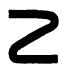
\includegraphics[keepaspectratio]{images/part001_1313f7e2.jpg}}

注记. --- 1) 若把假设 \(|\mathbf{f}_n| \leqslant g\) （其中 \(\mathrm{N}_p(g) < +\infty\) ）换成较弱的假设 \(\sup_{n} \mathrm{N}_p(\mathbf{f}_n) < +\infty\) ，定理 6 不再成立。例如，设 \(\mu\) 是 \(\mathbf{R}\) 上的 Lebesgue 测度；按下列方式定义连续函数 \(f_n\) ：\(f_n(x) = 0\) 对 \(x \leqslant 0\) 及对 \(x \geqslant \frac{2}{n}\) ，\(f_n(\frac{1}{n}) = n\) ，而 \(f_n\) 在区间 \([0, \frac{1}{n}]\) 与 \([\frac{1}{n}, \frac{2}{n}]\) 上是线性的。于是 \(\lim_{n \to \infty} f_n(x) = 0\) 对所有 \(x \in \mathbf{R}\) 成立，但 \(\mathrm{N}_1(f_n) = 1\) 对每个 \(n\) 成立（参见 §5, 习题 12）。

\pandocbounded{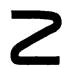
\includegraphics[keepaspectratio]{images/part001_8f7b1086.jpg}}

\begin{enumerate}
\def\labelenumi{\arabic{enumi})}
\setcounter{enumi}{1}
\tightlist
\item
  若不假定滤子 \(\mathfrak{F}\) 具有可数基，定理 6 的推论不再成立（参见 §1, No.~3, 定理 3 的推论后的注记 1）。
\end{enumerate}

\subsection{\texorpdfstring{空间 \(L_{F}^{p}\) （ \(1 \leqslant p < +\infty\) ）之间的关系}{空间 L sub F to the p （ 1 <= p < +infinity ）之间的关系}}

对每个实数 \(\alpha > 0\) ，映射 \(z \mapsto |z|^{\alpha-1} \cdot z\) 在 F 中 0 的余集上有定义且连续；此外，由于 \(\left||z|^{\alpha-1} \cdot z\right| = |z|^{\alpha}\) ，这个函数随 z 趋于 0，因而可以连续延拓到点 0，办法是给它在这个点处以值 0，即使 \(\alpha < 1\) 亦然。

定理 7. --- 设 p 与 q 是两个实数，使 \(1 \leqslant p < +\infty\) ，\(1 \leqslant q < +\infty\) 。若函数 f 属于 \(L_{F}^{p}\) ，则函数 \(|f|^{(p/q)-1} \cdot f\) 属于 \(L_{F}^{q}\) ，反之亦然。

按假设，存在具有紧支集的连续函数的序列 \((\mathbf{f}_{n})\) ，使 \(\sum_{n=1}^{\infty}\mathrm{N}_{p}(\mathbf{f}_{n})<+\infty\) 且 \(\mathbf{f}(x)=\sum_{n=1}^{\infty}\mathbf{f}_{n}(x)\) 几乎处处成立（No.~4, 定理 3）。令

\[
\mathbf {g} _ {n} = | \mathbf {f} _ {1} + \mathbf {f} _ {2} + \dots + \mathbf {f} _ {n} | ^ {(p / q) - 1} \cdot (\mathbf {f} _ {1} + \mathbf {f} _ {2} + \dots + \mathbf {f} _ {n});
\]

函数 \(g_{n}\) 具有紧支集且连续；另一方面，

\[
\left| \mathbf {g} _ {n} \right| ^ {q} = \left| \mathbf {f} _ {1} + \mathbf {f} _ {2} + \dots + \mathbf {f} _ {n} \right| ^ {p} \leqslant \left(\sum_ {n = 1} ^ {\infty} \left| \mathbf {f} _ {n} \right|\right) ^ {p} = h ^ {q},
\]

其中数值函数 \(h \geqslant 0\) （有限或非有限）满足不等式

\[
\left(\mathrm{N} _ {q} (h)\right) ^ {q} = \left(\mathrm{N} _ {p} \left(\sum_ {n = 1} ^ {\infty} | \mathbf {f} _ {n} |\right)\right) ^ {p} \leqslant \left(\sum_ {n = 1} ^ {\infty} \mathrm{N} _ {p} (\mathbf {f} _ {n})\right) ^ {p} <   + \infty
\]

此外，\(\mathbf{g}_n(x)\) 几乎处处趋于 \(\mathbf{g}(x) = |\mathbf{f}(x)|^{(p/q)-1} \cdot \mathbf{f}(x)\) ，因此 Lebesgue 定理表明 \(\mathbf{g} \in \mathcal{L}_{\mathrm{F}}^q\) 。逆命题是直接的，因为 \(\mathbf{f} = |\mathbf{g}|^{(q/p)-1} \cdot \mathbf{g}\) 。

可以证明映射 \(\mathbf{f} \mapsto |\mathbf{f}|^{\frac{p}{q}-1} \cdot \mathbf{f}\) 是 \(\mathcal{L}_{\mathrm{F}}^{p}\) 到 \(\mathcal{L}_{\mathrm{F}}^{q}\) 上的一个同胚（§6, 习题 10）。

推论 1. --- 为使函数 \(\mathbf{f}\) 属于 \(\mathcal{L}_{\mathrm{F}}^{p}\) ，必须且只须函数 \(|\mathbf{f}|^{p-1} \cdot \mathbf{f}\) 属于 \(\mathcal{L}_{\mathrm{F}}^{1}\) 。

推论 2. --- 为使正数值函数 f 属于 \(L^{p}\) ，必须且只须 \(f^{p}\) 属于 \(L^{1}\) 。

\pandocbounded{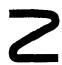
\includegraphics[keepaspectratio]{images/part001_881031c4.jpg}}

注意，若 \(f\) 是任意符号的数值函数，使 \(|f|^p\) 属于 \(\mathcal{L}^1\) ，则 \(f\) 不一定属于 \(\mathcal{L}^p\) （参见 §4, 习题 8）。

\section{可积函数与可积集}

\subsection{积分的延拓}

由空间 \(L_{F}^{p}\) 的定义可得：具有紧支集的连续函数所成的子空间 \(H_{F}\) 在 \(L_{F}^{p}\) 中稠密（§3, No.~4, 定义 2）。因此，每个连续的（对于 p 阶平均收敛拓扑）线性函数——定义在 \(H_{F}\) 上、取值于一个完备 Hausdorff 拓扑向量空间 G——都可以以唯一方式连续延拓为定义在 \(L_{F}^{p}\) 上、取值于 G 中的连续线性函数（GT, II, §3, No.~6, 定理 2 及 III, §3, No.~1, 命题 3）。

现在，对每个连续函数 \(\mathbf{f}\) （具有紧支集、取值于 Banach 空间 \(\mathrm{F}\) 的），我们已定义过（在 Ch. III, §3, No.~1）它的积分 \(\mu(\mathbf{f}) = \int \mathbf{f} d\mu\) （关于 \(\mu\) 的），它是 \(\mathrm{F}\) 的一个元素；而且我们已证明（Ch. III, §3, No.~2, 命题 6）不等式

\[
\left| \int \mathbf {f} d \mu \right| \leqslant \int | \mathbf {f} | d | \mu | = \mathrm{N} _ {1} (\mathbf {f}).\tag{1}
\]

这个不等式表明线性映射 \(\mathbf{f} \mapsto \int \mathbf{f} d\mu\) （\(\mathcal{H}_{\mathrm{F}}\) 到 \(\mathrm{F}\) 中的）对于 \(\mathcal{H}_{\mathrm{F}}\) 中的平均收敛拓扑是连续的。因此它可以连续延拓到整个空间 \(L_{F}^{1}\) ，从而我们可以给出下述定义：

定义 1. --- 属于 \(\mathcal{L}_{\mathrm{F}}^{1}(\mathrm{X},\mu)\) 的函数称为关于测度 \(\mu\) 可积的（或者再称它们是 \(\mu\) -可积的）。（关于 \(\mu\) 的）可积函数 \(\mathbf{f}\) 的积分，按定义是 \(\mathbf{f}\) 处所取的值，这个值是把一个线性映射连续延拓到 \(\mathcal{L}_{\mathrm{F}}^{1}\) 而得的，所说线性映射即 \(\mathbf{g} \mapsto \int \mathbf{g} d\mu\) （\(\mathcal{K}_{\mathrm{F}}\) 到 \(\mathrm{F}\) 中的）；它仍记作 \(\mu(\mathbf{f})\) 或 \(\int \mathbf{f} d\mu\) ，或 \(\int \mathbf{f}(x) d\mu(x)\) 或 \(\int \mathbf{f}\mu\) ，或 \(\int \mathbf{f}(x)\mu(x)\) 。

例子. --- 设 X 是一个离散空间，\(\mu\) 是 X 上的一个测度，并令 \(\alpha(x) = \mu(\varphi_{\{x\}})\) 对每个 \(x \in X\) 。此时 \(F_{F}^{1}\) 中的函数都是可积的，换句话说 \(L_{F}^{1} = F_{F}^{1}\) ；此外，对每个函数 \(f \in L_{F}^{1}\) ，

\[
\int \mathbf {f} d \mu = \sum_ {x \in X} \alpha (x) \mathbf {f} (x).
\]

因为，设 \(\mathbf{f} \in \mathcal{F}_F^1\) ；我们有 \(|\mu|^*(|\mathbf{f}|) = \sum_{x \in X} |\alpha(x)| \cdot |\mathbf{f}(x)| < +\infty\) （§1, No.~3, 例子）；于是对每个 \(\varepsilon > 0\) ，存在一个有限子集 \(M\) （\(X\) 的）使得

\[
\sum_ {x \in \mathrm{X} - \mathrm{M}} | \alpha (x) | \cdot | \mathbf {f} (x) | \leqslant \varepsilon .
\]

函数 \(\mathbf{g}\) 与 \(\mathbf{f}\) 在诸点 \(x\in M\) （\(|\mathbf{f}|\) 在那里为有限）处相等，在别处等于 0，它属于 \(\mathcal{H}(\mathrm{X};\mathrm{F})\) ，而且按已作的约定，

\[
| \mu | ^ {*} (| \mathbf {f} - \mathbf {g} |) \leqslant \sum_ {\boldsymbol {x} \in \mathrm{X} - \mathrm{M}} | \alpha (\boldsymbol {x}) | \cdot | \mathbf {f} (\boldsymbol {x}) | \leqslant \varepsilon ,
\]

这就证明了 \(\mathbf{f} \in \mathcal{L}_{\mathrm{F}}^{1}\) 。另一方面，

\[
\left| \mu (\mathbf {g}) - \sum_ {x \in X} \alpha (x) \mathbf {f} (x) \right| \leqslant \sum_ {x \in X - M} | \alpha (x) | \cdot | \mathbf {f} (x) | \leqslant \varepsilon ,
\]

由此得第二个断言。

换句话说，\(\mu\) -可积函数 \(\mathbf{f}\) 就是使族 \((\alpha(x)\mathbf{f}(x))_{x\in X}\) 绝对可和（GT, IX, §3, No.~6）的那些函数，且积分 \(\int \mathbf{f} d\mu\) 是这个族的和。

由于 \(\mu(\mathbf{f})\) 依定义在 \(\mathcal{L}_{\mathrm{F}}^{1}\) 上连续，且它取值于一个 Hausdorff 空间，故 \(\mu(\mathbf{f}) = 0\) 对每个属于 0 在 \(\mathcal{L}_{\mathrm{F}}^{1}\) 中的闭包的函数（即可忽略的函数）成立；若 \(\mathbf{f}\) 与 \(\mathbf{g}\) 是两个等价的可积函数，则 \(\mu(\mathbf{f}) = \mu(\mathbf{g})\) 。换句话说，\(\mu(\mathbf{f})\) 的值只依赖于类 \(\widetilde{\mathbf{f}}\) （可积函数 \(\mathbf{f}\) 的）；它仍记作 \(\mu(\widetilde{\mathbf{f}})\) ，而函数 \(\widetilde{\mathbf{f}} \mapsto \mu(\widetilde{\mathbf{f}})\) 是 \(L_{F}^{1}\) 到 F 中的一个连续线性映射。若一个取值于 F、在 X 中几乎处处有定义的函数 f 等价于一个可积函数，我们仍说 f 是可积的，并写 \(\int f d\mu = \mu(\widetilde{\mathbf{f}})\) ；类似地可定义取值于 \(\overline{R}\) 、几乎处处有定义且有限的可积函数及其积分。

\subsection{积分的性质}

命题 1. --- 对每个正的 \(\mu\) -可积数值函数 \(f\) ，

\[
\int f d | \mu | = \int^ {*} f d | \mu | = \mathrm{N} _ {1} (f) \geqslant 0.\tag{2}
\]

因为，\(\int f d|\mu|\) 与 \(\mathrm{N}_{1}(f)\) 都在 \(L^{1}\) 上连续，且对每个具有紧支集的连续函数 \(f \geqslant 0\) 相等；另一方面，每个函数 \(f \geqslant 0\) （\(L^{1}\) 中的）都是具有紧支集的连续函数 \(\geqslant 0\) 的序列的极限（就平均收敛意义而言）（ \(\S3\) , No.~5, 命题 11）；由此得命题。

推论 1. --- 对每个可积函数 \(\mathbf{f} \in \mathcal{L}_{\mathrm{F}}^{1}\) ，\(|\mathbf{f}|\) 是可积的，且

\[
\int | \mathbf {f} | d | \mu | = \int^ {*} | \mathbf {f} | d | \mu | = \mathrm{N} _ {1} (\mathbf {f}).\tag{3}
\]

我们将经常使用命题 1 及其推论 1，即把 \(\int^{*}fd|\mu|\) 或 \(\mathrm{N}_{1}(f)\) 换成 \(\int fd|\mu|\) ，当所处理的是可积函数 \(\geqslant 0\) 时。例如，为使两个可积函数 \(\mathbf{f},\mathbf{g}\) 等价，必须且只须 \(\int |\mathbf{f} - \mathbf{g}|d|\mu| = 0\) 。

我们回顾，为使函数 \(\mathbf{f}\) 属于 \(\mathcal{L}_{\mathrm{F}}^{p}\) ，必须且只须函数 \(|\mathbf{f}|^{p - 1}\cdot \mathbf{f}\) 属于 \(\mathcal{L}_{\mathrm{F}}^{1}\) （§3, No.~8, 定理 7 的推论 1），即它是可积的；这正是术语« \(p\) 次幂可积函数»的来由。此外：

推论 2. --- 对每个函数 \(\mathbf{f} \in \mathcal{L}_{\mathrm{F}}^{p}\) ，数值函数 \(|\mathbf{f}|^{p}\) 是可积的，且

\[
\mathrm{N} _ {p} (\mathbf {f}) = \left(\int | \mathbf {f} | ^ {p} d | \mu |\right) ^ {1 / p}.\tag{4}
\]

这由 \(|\mathbf{f}|\) 属于 \(\mathcal{L}^p\) （§3, No.~5, 命题 11）这一事实以及公式 (2) 立得。

命题 2. --- 对每个可积函数 f，

\[
\left| \int \mathbf {f} d \mu \right| \leqslant \int | \mathbf {f} | d | \mu |.\tag{5}
\]

由不等式 (1) 通过取极限，并注意到 (3) 以及 \(\mathrm{N}_{1}(\mathbf{f})\) 在 \(L_{F}^{1}\) 上的连续性，立得此式。

定理 1. --- 设 F 与 G 是两个 Banach 空间，u 是 F 到 G 中的一个连续线性映射。对每个取值于 F 的可积函数 f，\(u \circ f\) 是可积的，且

\[
\int \mathbf {u} (\mathbf {f} (x)) d \mu (x) = \mathbf {u} \left(\int \mathbf {f} (x) d \mu (x)\right).\tag{6}
\]

我们已知 \(\mathbf{u} \circ \mathbf{f}\) 是可积的（§3, No.~5, 定理 4）；关系式 (6) 对每个 \(\mathbf{f} \in \mathcal{K}_{\mathrm{F}}\) 成立，故由恒等延拓原理推广到每个可积函数 \(\mathbf{f}\) ：因为 \(\mathbf{f} \mapsto \mathbf{u} \circ \mathbf{f}\) 对于平均收敛拓扑是连续的，这由不等式 \(\mathrm{N}_1(\mathbf{u} \circ \mathbf{f}) \leqslant \| \mathbf{u} \| \cdot \mathrm{N}_1(\mathbf{f})\) 得出。

推论 1. --- 设 \(\mathbf{a}'\) 是 \(\mathbf{F}\) 上的一个连续线性形式。若 \(\mathbf{f}\) 是取值于 \(\mathbf{F}\) 的一个可积函数，则数值函数 \(\langle \mathbf{f}, \mathbf{a}' \rangle\) 是可积的，且

\[
\int \left\langle \mathbf {f} (x), \mathbf {a} ^ {\prime} \right\rangle d \mu (x) = \left\langle \int \mathbf {f} (x) d \mu (x), \mathbf {a} ^ {\prime} \right\rangle .\tag{7}
\]

我们将在 Ch. VI, §1, 习题 7、11 与 12 中看到，可以存在函数 \(\mathbf{f}\) ，取值于一个无穷维 Banach 空间 \(\mathbf{F}\) ，使 \(\langle \mathbf{f}, \mathbf{a}' \rangle\) 对每个连续线性形式 \(\mathbf{a}'\) （\(\mathbf{F}\) 上的）都可积，而 \(\mathbf{f}\) 本身不可积。

推论 2. --- 若 \(\mathbf{a}_k\) （ \(1 \leqslant k \leqslant n\) ）是 F 中的向量，而 \(f_k\) （ \(1 \leqslant k \leqslant n\) ）是可积数值函数，则函数 \(\mathbf{f} = \sum_{k=1}^{n} \mathbf{a}_k f_k\) 是可积的，且

\[
\int \left(\sum_ {k = 1} ^ {n} \mathbf {a} _ {k} f _ {k}\right) d \mu = \sum_ {k = 1} ^ {n} \mathbf {a} _ {k} \int f _ {k} d \mu .\tag{8}
\]

\subsection{积分中取极限}

命题 3. --- 设 B 是 \(L_{F}^{1}\) 上的一个滤子基。假定存在紧集 \(K \subset X\) ，使对每个集 \(M \in B\) ，所有函数 \(f \in M\) 的支集都含于 K。在这些条件下，若 B 在 X 上一致收敛于 \(f_{0}\) ，则函数 \(f_{0}\) 是可积的，且

\[
\int \mathbf {f} _ {0} d \mu = \lim _ {\mathfrak {B}} \int \mathbf {f} d \mu .\tag{9}
\]

因为，\(\mathfrak{B}\) 平均收敛于 \(\mathbf{f}_0\) （§3, No.~3, 命题 4）。

命题 4. --- 设 \((f_n)\) 是可积数值函数的一个递增（相应地，递减）序列。为使序列的上（相应地，下）包络 \(f\) 可积，必须且只须 \(\sup_{n} \int f_n d|\mu| < +\infty\) （相应地 \(\inf_{n} \int f_n d|\mu| > -\infty\) ）；此时

\[
\int f d \mu = \lim _ {n \to \infty} \int f _ {n} d \mu .\tag{10}
\]

我们只考虑递增序列。序列 \(g_{n} = f_{n} + f_{1}^{-}\) 是递增的，由可积函数 \(\geqslant 0\) 组成；由于它的上包络是 \(g = f + f_{1}^{-}\) ，命题由 §3, No.~6 的定理 5 得出。

定理 2. --- 设 A 是一个指标集，由具有可数基的滤子 F 过滤。设 \((\mathbf{f}_{\alpha})_{\alpha\in\mathrm{A}}\) 是可积函数的一个族，它关于滤子 F 几乎处处逐点收敛于一个函数 f；若存在数值函数 \(g\geqslant0\) 使 \(\int^{*}gd|\mu|<+\infty\) 且 \(|\mathbf{f}_{\alpha}(x)|\leqslant g(x)\) 在 X 中几乎处处成立对每个 \(\alpha\in A\) ，则函数 f 是可积的，且

\[
\int \mathbf {f} d \mu = \lim _ {\mathfrak {F}} \int \mathbf {f} _ {\alpha} d \mu .\tag{11}
\]

定理由 Lebesgue 定理（§3, No.~7, 定理 6 的推论）得出，因为在陈述的条件下，\(\mathbf{f}_{\alpha}\) 平均收敛于 \(\mathbf{f}\) （关于 \(\mathfrak{F}\) ）。

推论 1. --- 设 \(\Omega\) 是一个拓扑空间，\(t_0\) 是 \(\Omega\) 的一个具有可数基本邻域系的点，\(\mathbf{f}\) 是 \(\mathbf{X} \times \Omega\) 到 \(\mathbf{F}\) 中的一个映射，具有下列性质：

\begin{enumerate}
\def\labelenumi{\alph{enumi})}
\item
  对每个 \(t \in \Omega\) ，函数 \(x \mapsto \mathbf{f}(x, t)\) 是可积的；
\item
  对每个 \(x \in \mathrm{X}\) ，函数 \(t \mapsto \mathbf{f}(x, t)\) 在 \(t_0\) 处连续；
\item
  存在 \(t_0\) 的一个邻域 U 与定义在 X 上的数值函数 \(g \geqslant 0\) ，使 \(\int^{*} g d|\mu| < +\infty\) 且 \(|\mathbf{f}(x,t)| \leqslant g(x)\) 对所有 \(x \in X\) 与 \(t \in U\) 成立。
\end{enumerate}

在这些条件下，映射 \(t \mapsto \int \mathbf{f}(x,t) d\mu(x)\) （\(\Omega\) 到 \(\mathbf{F}\) 中的）在点 \(t_0\) 处连续。

推论 2. --- 设 \((\mathbf{f}_{n})\) 是可积函数的一个序列，使通项为 \(\mathbf{f}_{n}(x)\) 的级数几乎处处收敛；若存在函数 \(g \geqslant 0\) 使 \(\int^{*} g d|\mu| < +\infty\) 且对每个整数 n 有 \(\left|\sum_{k=1}^{n} \mathbf{f}_{k}(x)\right| \leqslant g(x)\) 几乎处处成立，则和 \(\mathbf{f}(x)\) （通项为 \(\mathbf{f}_{n}(x)\) 的级数的，几乎处处有定义的）是可积的，且

\[
\int \mathbf {f} d \mu = \sum_ {n = 1} ^ {\infty} \int \mathbf {f} _ {n} d \mu\tag{12}
\]

（«级数的逐项积分»）。

\subsection{可积数值函数的特征}

命题 5. --- 为使数值函数 \(f \geqslant 0\) （有限或非有限，在 X 上是下半连续的）可积，必须且只须 \(\int^{*} f d|\mu| < +\infty\) 。

一切归结为证明条件是充分的。\(|\mu|^*(f)\) 的定义（§1, No.~1, 定义 1）表明，对每个 \(\varepsilon > 0\) ，存在连续函数 \(g \geqslant 0\) ，具有紧支集，使 \(g \leqslant f\) 且 \(|\mu|^*(f) \leqslant |\mu|(g) + \varepsilon\) 。但 \(f - g\) 是下半连续的且 \(\geqslant 0\) ，因此（§1, No.~1, 定理 2）

\[
| \mu | ^ {*} (f) = | \mu | (g) + | \mu | ^ {*} (f - g),
\]

换句话说 \(\mathrm{N}_{1}(f-g)=|\mu|^{*}(f-g)=|\mu|^{*}(f)-|\mu|(g)\leqslant\varepsilon\) ，这就证明了 f 是可积的（§3, No.~4, 命题 7）。

推论 1. --- 为使有限数值函数 \(f \geqslant 0\) （在 X 上是上半连续的）可积，必须且只须 \(\int^{*} f d|\mu| < +\infty\) 。

因为，若 \(|\mu|^*(f) < +\infty\) ，则存在下半连续函数 \(h\) 使 \(f \leqslant h\) 且 \(|\mu|^*(h) < +\infty\) ；\(h - f\) 处处有定义且是下半连续的，且 \(|\mu|^*(h - f) \leqslant |\mu|^*(h) < +\infty\) ；因此 \(h - f\) 是可积的，而由于 \(f(x) = h(x) - (h(x) - f(x))\) 几乎处处成立，\(f\) 是可积的。

推论 2. --- 设 H 是一个非空集，由下半（相应地，上半）连续且可积的数值函数组成，按关系 \(\leqslant (\text{resp. } \geqslant)\) 有向；若

\[
\sup _ {f \in \mathrm{H}} \int f d | \mu | <   + \infty \quad (\mathrm{resp.} \inf _ {f \in \mathrm{H}} \int f d | \mu | > - \infty),
\]

则 H 的上（相应地，下）包络 g 是可积的，

\[
\int g d \mu = \lim _ {f \in \mathrm{H}} \int f d \mu ,
\]

且 \(\int g d|\mu| = \sup_{f\in \mathrm{H}}\int f d|\mu|\) （相应地 \(\int g d|\mu| = \inf_{f\in \mathrm{H}}\int f d|\mu|\) ）。

我们可以只限于下半连续函数的情形；函数 \(f^{+}\) （相应地 \(f^{-}\) ），当 \(f\) 遍历 \(\mathbf{H}\) 时，构成一个按 \(\leqslant (\text{resp. } \geqslant)\) 有向的下半（相应地，上半）连续函数 \(\geqslant 0\) 所成之集；诸 \(f^{+}\) （相应地 \(f^{-}\) ）（对 \(f \in \mathbf{H}\) ）的上（相应地，下）包络等于 \(g^{+}\) （相应地 \(g^{-}\) ）。另一方面，可以把 \(\mathbf{H}\) 换成它的一个截段（它对 H 是共尾的），即由那些 \(f \in \mathbf{H}\) （它们 \(\geqslant f_{0}\) ）组成，其中 \(f_{0} \in \mathbf{H}\) 是某个函数；此时 \(\int f^{+} d|\mu| \leqslant \int f d|\mu| + \int f_{0}^{-} d|\mu|\) ；于是我们看到，当 \(\mathbf{H}\) 由正函数组成时，我们归结为证明推论的两个断言。若 \(\mathbf{H}\) 按 \(\leqslant\) 有向且由下半连续函数 \(\geqslant 0\) 组成，则我们已知（§1, No.~1, 定理 1）

\[
| \mu | ^ {*} (g) = \sup _ {f \in \mathrm{H}} | \mu | ^ {*} (f) = \sup _ {f \in \mathrm{H}} \int f d | \mu | <   + \infty ,
\]

因此 g 是下半连续的，由命题 5 知它可积；我们有 \(\int g d|\mu| = \lim_{f \in H} \int f d|\mu|\) ，且由于 \(f \leqslant g\) ，\(\lim_{f \in H} N_1(g - f) = 0\) ，这表明 f 关于 H 平均收敛于 g，从而在这种情形证明了推论。若 H 按 \(\geqslant\) 有向，由上半连续可积函数 f 组成，使 \(0 \leqslant f \leqslant f_1\) （\(f_1 \in H\) 的），则存在下半连续可积函数 h 使 \(f_1 \leqslant h\) ；我们可以写 \(f = h - f'\) ，其中 \(f'(x) = h(x) - f(x)\) 当 \(f(x) < +\infty\) 时成立，而 \(f'(x) = 0\) 否则。显然诸 \(f'\) 构成一个按 \(\leqslant\) 有向的下半连续可积函数 \(\geqslant 0\) 所成之集，且

\[
\int f ^ {\prime} d | \mu | \leqslant \int h d | \mu | <   + \infty ;
\]

我们可以对它们应用前面已证明的结果；若 \(g'\) 是诸 \(f'\) 的上包络，则 h 与 \(g'\) 都几乎处处有限，因此 \(h - g'\) 几乎处处有定义且几乎处处等于 g；由此，推论的结论在这种情形立得。

推论 3. --- 设 \(f\) 是一个有界数值函数，在 \(X\) 上是上半连续的且具有紧支集。则映射 \(\mu \mapsto \int f d\mu\) 在 \(\mathcal{M}_{+}(X)\) 上对于淡拓扑是上半连续的。

若 \(h\) 是 \(\mathcal{H}_{+}(\mathrm{X})\) 中的一个函数，使 \(|f| \leqslant h\) （Ch. III, §1, No.~2, 引理 1），则 \(0 \leqslant f + h \leqslant 2h\) ，且由于 \(f + h\) 是上半连续的，由推论 1 知 \(f\) 是 \(\mu\) -可积的对每个测度 \(\mu\) （\(\mathrm{X}\) 上的）。此外，\(\mu(f) = \mu(h) - \mu(h - f)\) ，而 \(h - f\) 是下半连续函数 \(\geqslant 0\) 。由于映射 \(\mu \mapsto \mu(h - f)\) 在 \(\mathcal{M}_{+}(\mathrm{X})\) 上对于淡拓扑是下半连续的（§1, No.~1, 命题 4），这就证明了推论。

定理 3. --- 为使数值函数 \(f \geqslant 0\) 可积，必须且只须：对每个 \(\varepsilon > 0\) ，存在上半连续函数 \(g \geqslant 0\) （取有限值且具有紧支集）与下半连续可积函数 \(h\) ，使 \(g \leqslant f \leqslant h\) 且 \(\int (h - g) d|\mu| \leqslant \varepsilon\) 。

条件是充分的，这由可积性的一般判别法（§3, No.~4, 命题 8）、命题 5 及其推论 1 得出。我们来证明条件是必要的。若 \(f \geqslant 0\) 可积，则对每个 \(\varepsilon > 0\) ，存在函数 \(u \geqslant 0\) ，连续且具有紧支集，使 \(\mathrm{N}_1(f - u) \leqslant \varepsilon / 4\) 。依 \(\mathrm{N}_1\) 的定义，这蕴涵存在下半连续函数 \(v \geqslant 0\) 使 \(|\mu|^*(v) \leqslant \varepsilon / 2\) 且 \(|f - u| \leqslant v\) 。于是 \(-v(x) \leqslant f(x) - u(x) \leqslant v(x)\) 对所有 \(x \in X\) 成立，且由于 \(u(x)\) 处处有限，得出 \((u(x) - v(x))^+ \leqslant f(x) \leqslant u(x) + v(x)\) 对所有 \(x \in X\) 成立。函数 \(g = (u - v)^+\) 与 \(h = u + v\) 满足要求。

推论. --- 对每个可积（相应地，可积且 \(\geqslant0\) ）的数值函数 f，存在上半连续可积函数的一个递增序列 ( \(g_{n}\) ) （相应地，这些函数可积、取有限值 \(\geqslant0\) 且具有紧支集），以及下半连续可积函数的一个递减序列 ( \(h_{n}\) ) ，使得：

\(1^{\circ} g_{n}(x) \leqslant f(x) \leqslant h_{n}(x)\) 对所有 \(x \in X\) 与每个整数 \(n\) 成立；

\(2^{\circ} f(x)\) 几乎处处等于序列 \((h_{n})\) 的下包络 h 与序列 \((g_{n})\) 的上包络 g；

\[
3 ^ {\circ} \int f d \mu = \lim _ {n \rightarrow \infty} \int g _ {n} d \mu = \lim _ {n \rightarrow \infty} \int h _ {n} d \mu .
\]

首先设 \(f \geqslant 0\) 。由定理 3，对每个 n 存在下半连续可积函数 \(v_{n}\) 与上半连续函数 \(u_{n} \geqslant 0\) （取有限值且具有紧支集），使得

\[
u _ {n} \leqslant f \leqslant v _ {n} \quad \text { and } \quad \int (v _ {n} - u _ {n}) d | \mu | \leqslant 1 / n;
\]

令 \(g_{n} = \sup(u_{1}, u_{2}, \ldots, u_{n})\) 与 \(h_{n} = \inf(v_{1}, v_{2}, \ldots, v_{n})\) ，则序列 \((g_{n})\) 与 \((h_{n})\) 满足要求。因为，由于 \(g \leqslant f\) ，g 由 No.~3 的命题 4 知是可积的；又由于

\[
\int (f - g _ {n}) d | \mu | \leqslant \int (v _ {n} - u _ {n}) d | \mu | \leqslant 1 / n
\]

由此有

\[
\int (f - g) d | \mu | = \lim _ {n \rightarrow \infty} \int (f - g _ {n}) d | \mu | = 0
\]

（No.~3, 命题 4），这就证明了 \(f\) 与 \(g\) 等价。对序列 \((h_n)\) 可类似论证。

若 \(f\) 不是正的，我们可以把上述结果应用于 \(f^{+}\) 与 \(f^{-}\) ，于是有两个递增序列 \((g_n')\) 、\((g_n'')\) （上半连续可积函数的）与两个递减序列 \((h_n')\) 、\((h_n'')\) （下半连续可积函数的），使得：\(1^\circ g_n' \leqslant f^{+} \leqslant h_n'\) ，\(g_n'' \leqslant -f^{-} \leqslant h_n''\) ；\(2^\circ f^{+}\) （相应地 \(-f^{-}\) ）几乎处处等于诸 \(g_n'\) 的上包络与诸 \(h_n'\) 的下包络（相应地，等于诸 \(g_n''\) 的上包络与诸 \(h_n''\) 的下包络）；以及 \(3^\circ\) ：

\[
\begin{array}{r} \int f ^ {+} d \mu = \lim _ {n \to \infty} \int g _ {n} ^ {\prime} d \mu = \lim _ {n \to \infty} \int h _ {n} ^ {\prime} d \mu , \\ - \int f ^ {-} d \mu = \lim _ {n \to \infty} \int g _ {n} ^ {\prime \prime} d \mu = \lim _ {n \to \infty} \int h _ {n} ^ {\prime \prime} d \mu . \end{array}
\]

此外，我们可以假定诸 \(g_{n}^{\prime}\) 与诸 \(h_{n}^{\prime\prime}\) 处处有限；此时显然序列 \(g_{n}=g_{n}^{\prime}+g_{n}^{\prime\prime}\) 与 \(h_{n}=h_{n}^{\prime}+h_{n}^{\prime\prime}\) 满足要求。

由 No.~3 的定理 2；于是积分 \(\int_{-\infty}^{+\infty} \mathbf{f}(x) dx\) 是绝对收敛的（FRV, II, §2, No.~3）。此外，\(\int \mathbf{f} d\mu = \int_{-\infty}^{+\infty} \mathbf{f}(x) dx\) 由 No.~3 的定理 2 得出。反之，设 \(\int_{-\infty}^{+\infty} \mathbf{f}(x) dx\) 绝对收敛；仍由 No.~3 的定理 2，\(\int \mathbf{f} d\mu = \int_{-\infty}^{+\infty} \mathbf{f}(x) dx\) 。注意，若积分 \(\int_{-\infty}^{+\infty} \mathbf{f}(x) dx\) 收敛而非绝对收敛；则 \(\mathbf{f}\) 关于 Lebesgue 测度不可积。

\begin{enumerate}
\def\labelenumi{\arabic{enumi})}
\setcounter{enumi}{1}
\tightlist
\item
  把 No.~3 的命题 3 应用于 Lebesgue 测度与正则函数，便重新得出关于紧区间上正则函数积分取极限的定理（FRV, II, §3, No.~1, 命题 1）；对正则函数的序列（或具有可数基的滤子），No.~3 的定理 2 大大改进了该命题，因为对紧区间上一致有界的正则函数，它以逐点收敛代替一致收敛（参见 §5, No.~4, 定理 2）。然而，关于非紧区间上正则函数绝对收敛积分的取极限，我们注意 No.~3 定理 2 的条件蕴涵所考虑的积分是一致收敛的（按 FRV, II, §3, No.~2 中定义的意义），因而除涉及函数 \(\mathbf{f}_{\alpha}\) 在每个紧区间上的收敛外，并不改进第 IV 卷（loc. cit.）中给出的收敛条件。最后，对正则函数非绝对收敛积分所给出的取极限条件，仍然超出本章展开的理论范围。
\end{enumerate}

\subsection{可积集}

定义 2. --- 局部紧空间 X 的子集 A 称为关于 X 上的测度 \(\mu\) 可积的（或称它是 \(\mu\) -可积的），如果 A 的特征函数 \(\varphi_{A}\) 可积。有限数 \(\mu(A) = \int \varphi_{A} d\mu\) 称为 A 的测度。

对每个可积集 A，\(|\mu|(A) = |\mu|^{*}(A)\) （No.~2, 命题 1）；为使一个集是可忽略的，必须且只须它关于 \(|\mu|\) 的测度为零。

命题 6. --- 可积集的有限族 \((\mathrm{A}_{i})_{1\leqslant i\leqslant n}\) 的并集是可积的，且

\[
| \mu | \left(\bigcup_ {i = 1} ^ {n} \mathrm{A} _ {i}\right) \leqslant \sum_ {i = 1} ^ {n} | \mu | (\mathrm{A} _ {i}).\tag{13}
\]

此外，若诸 \(\mathrm{A}_i\) 两两不相交，则

\[
\mu \left(\bigcup_ {i = 1} ^ {n} \mathrm{A} _ {i}\right) = \sum_ {i = 1} ^ {n} \mu (\mathrm{A} _ {i}).\tag{14}
\]

因为，若 \(\mathbf{A} = \bigcup_{i=1}^{n} \mathbf{A}_i\) ，则 \(\varphi_{\mathbf{A}} = \sup \varphi_{\mathbf{A}_i}\) ，因此（§3, No.~5, 命题 12 的推论）若诸 \(\mathbf{A}_i\) 可积，则 \(\mathbf{A}\) 也可积；关系式 (13) 是外测度的类似关系式（§1, No.~4, 命题 18）的特例，只需注意到关系式 \(|\mu|(\mathrm{A}) = |\mu|^*(\mathrm{A})\) ；最后，若诸 \(\mathbf{A}_i\) 两两不相交，则 \(\varphi_{\mathrm{A}} = \sum_{i=1}^{n} \varphi_{\mathrm{A}_i}\) ，由此得 (14)。

命题 7. --- \(1^{\circ}\) 若 A 与 B 是两个可积集，使 \(\mathbf{B} \subset \mathbf{A}\) ，则集 \(\mathbf{C} = \mathbf{A} - \mathbf{B}\) 是可积的，且

\[
\mu (\mathrm{C}) = \mu (\mathrm{A}) - \mu (\mathrm{B}).\tag{15}
\]

\(2^{\circ}\) 可积集的可数族的交是可积的。第一部分由 \(\varphi_{\mathrm{C}} = \varphi_{\mathrm{A}} - \varphi_{\mathrm{B}}\) 这一事实得出。另一方面，若 \((\mathbf{A}_n)\) 是可积集的一个序列而 A 是它们的交，则 \(\varphi_{\mathrm{A}} = \inf_{n} \varphi_{\mathrm{A}_n}\) ，因此 A 是可积的（No.~3, 命题 4）。

推论. --- 若 \((\mathrm{A}_{n})\) 是可积集的一个递减序列，则 \(\mu(\bigcap_{n}\mathrm{A}_{n})=\lim_{n\to\infty}\mu(\mathrm{A}_{n})\) 。

因为，若 \(\mathrm{A} = \bigcap_{n}\mathrm{A}_{n}\) ，则 \(\varphi_{\mathrm{A}}\) 是递减序列 \((\varphi_{\mathrm{A}_n})\) 的下包络（No.~3, 命题 4）。

命题 8. --- 设 \((\mathbf{A}_{n})\) 是可积集的一个递增序列；为使并集 \(A = \bigcup_{n} A_{n}\) 可积，必须且只须 \(\sup_{n} |\mu|(\mathbf{A}_{n}) < +\infty\) ；此时

\[
\mu (\mathrm{A}) = \lim _ {n \rightarrow \infty} \mu (\mathrm{A} _ {n}).\tag{16}
\]

因为，诸 \(\varphi_{\mathrm{A}_n}\) 构成可积函数的一个递增序列，且 \(\varphi_{\mathrm{A}} = \sup_n \varphi_{\mathrm{A}_n}\) ；于是命题由 No.~3 的命题 4 得出。

推论. --- 设 \((\mathrm{A}_{n})\) 是可积集的一个序列，使 \(\sum_{n=1}^{\infty} |\mu|(\mathrm{A}_{n}) < +\infty\) ；则并集 \(A = \bigcup_{n} A_{n}\) 是可积的，且

\[
| \mu | \left(\bigcup_ {n} \mathrm{A} _ {n}\right) \leqslant \sum_ {n = 1} ^ {\infty} | \mu | (\mathrm{A} _ {n}).\tag{17}
\]

因为，\(\varphi_{\mathrm{A}} = \sup_n\varphi_{\mathrm{A}_n}\) ，且

\[
| \mu | ^ {*} (\mathrm{A}) \leqslant \sum_ {n = 1} ^ {\infty} | \mu | ^ {*} (\mathrm{A} _ {n}) = \sum_ {n = 1} ^ {\infty} | \mu | (\mathrm{A} _ {n}) <   + \infty
\]

（§1, No.~4, 命题 18）；因此 A 是可积的（§3, No.~6, 定理 5 的推论 2），且由于 \(|\mu|(\mathrm{A}) = |\mu|^*(\mathrm{A})\) ，我们确有 (17)。

命题 9. --- 设 \((\mathbf{A}_{n})\) 是两两不相交的可积集的一个序列，使 \(\sum_{n=1}^{\infty}|\mu|(\mathbf{A}_{n})<+\infty\) ；则

\[
\mu \left(\bigcup_ {n} \mathrm{A} _ {n}\right) = \sum_ {n = 1} ^ {\infty} \mu (\mathrm{A} _ {n}).\tag{18}
\]

因为，若 \(\mathbf{A} = \bigcup_{n}\mathbf{A}_{n}\) ，则 \(\varphi_{\mathrm{A}} = \sum_{n = 1}^{\infty}\varphi_{\mathrm{A}_n}\) ，于是命题由 (17) 与 No.~3 定理 2 的推论 2 得出。

关系式 (18) 也可表述为：测度 \(\mu\) 在 X 的可积子集所成的集合上是完全可加的。

\subsection{集合可积性的判别法}

命题 10. --- 为使 X 中的开（相应地，闭）集 A 可积，必须且只须 \(|\mu|^{*}(A)<+\infty\) 。

由于此时 \(\varphi_{A}\) 是下半（相应地，上半）连续的，命题由 No.~4 的命题 5 及其推论 1 得出。

推论 1. --- 每个紧集都是可积的；每个相对紧的开集都是可积的。

推论 2. --- 对 X 上的每个正测度 \(\mu\) ，A \(\mapsto\) \(\mu^{*}(\mathrm{A})\) 是 X 上的一个容量（参见 GT, IX, §6, No.~9, 例子）。

例子. --- 对 R 上的 Lebesgue 测度 \(\mu\) ，由命题 10 知每个有界开区间 {]}a,b{[} 都是可积的且测度为 b-a（§1, No.~2, 命题 9）。由于每个退缩为一点的集对 Lebesgue 测度都是可忽略的，于是以 a 与 b 为端点的所有区间都有相同的测度 b-a。

命题 11. --- 设 \(\mathfrak{G}\) 是 X 中可积开集所成的一个集，按关系 \(\subset\) 有向；为使 \(A = \bigcup_{G \in \mathfrak{G}} G\) 可积，必须且只须 \(\sup_{G \in \mathfrak{G}} |\mu|(G) < +\infty\) ；此时 \(\mu(A) = \lim_{\mathfrak{G}} \mu(G)\) 且 \(|\mu|(A) = \sup_{G \in \mathfrak{G}} |\mu|(G)\) 。

因为，已知 \(|\mu|^*(\mathbf{A}) = \sup_{\mathbf{G} \in \mathfrak{G}} |\mu|(\mathbf{G})\) （§1, No.~2, 命题 7）；于是命题由命题 10 得出。

推论. --- 设 \(\mathfrak{F}\) 是 X 中可积闭集所成的一个集，按关系 \(\supset\) 有向；则闭集 \(B = \bigcap_{H \in \mathfrak{F}} H\) 是可积的，且有 \(\mu(B) = \lim_{\mathfrak{F}} \mu(H)\) 与 \(|\mu|(B) = \inf_{H \in \mathfrak{F}} |\mu|(H)\) 。

因为，设 \(H_{0}\) 是 F 中的一个集；由于 \(H_{0}\) 可积，它含于一个可积开集 U 中（§1, No.~4, 命题 19）；开集 \(U \cap CH\) 构成一个按关系 \(\subset\) 有向的集，它们都含于 U 中，且并集为 \(U \cap CB\) ；于是我们归结为命题 11。

定理 4. --- 为使一个集 A 可积，必须且只须：对每个 \(\varepsilon > 0\) ，存在可积开集 G 与紧集 K，使 \(K \subset A \subset G\) 且

\[
| \mu | (\mathrm{G} - \mathrm{K}) = | \mu | (\mathrm{G}) - | \mu | (\mathrm{K}) \leqslant \varepsilon .
\]

\begin{enumerate}
\def\labelenumi{\alph{enumi})}
\item
  条件是充分的，因为它意味着 \(\varphi_{\mathrm{K}} \leqslant \varphi_{\mathrm{A}} \leqslant \varphi_{\mathrm{G}}\) 且 \(\int (\varphi_{\mathrm{G}} - \varphi_{\mathrm{K}}) d|\mu| \leqslant \varepsilon\) ；由于 \(\varphi_{\mathrm{G}}\) 与 \(\varphi_{\mathrm{K}}\) 可积，\(\varphi_{\mathrm{A}}\) 也可积（§3, No.~4, 命题 8）。
\item
  条件是必要的。若 A 可积，则存在开集 \(G \supset A\) 使 \(|\mu|^{*}(G)\) 可任意接近 \(|\mu|^{*}(A) = |\mu|(A)\) （§1, No.~4, 命题 19）；于是，一切归结为证明：对每个 \(\varepsilon > 0\) ，存在紧集 \(K \subset A\) 使 \(|\mu|(A) - |\mu|(K) \leqslant \varepsilon\) 。由于 \(\varphi_{A}\) 可积，存在函数 \(f \geqslant 0\) ，上半连续且具有紧支集 S，使 \(f \leqslant \varphi_{A}\) 且 \(\int(\varphi_{A} - f)d|\mu| \leqslant \varepsilon/2\) （No.~4, 定理 3）。设 \(\delta > 0\) 是任意一个数，并设 K 是点 \(x \in X\) （使 \(f(x) \geqslant \delta\) 的）所成之集；K 是闭的且含于 S 中，因而是紧的，且由于 \(f \leqslant \varphi_{A}\) ，我们有 \(K \subset A\) 。集 B = A - K 是可积的，且 \(f \leqslant \varphi_{K} + \delta\varphi_{B}\) ，由此
\end{enumerate}

\[
\int f d | \mu | \leqslant | \mu | (\mathrm{K}) + \delta \cdot | \mu | (\mathrm{B}) \leqslant | \mu | (\mathrm{K}) + \delta \cdot | \mu | (\mathrm{A}),
\]

最后

\[
| \mu | (\mathrm{A}) \leqslant \int f d | \mu | + \frac {\varepsilon}{2} \leqslant | \mu | (\mathrm{K}) + \delta \cdot | \mu | (\mathrm{A}) + \frac {\varepsilon}{2},
\]

这就完成了证明，因为 \(\delta\) 是任意的。

推论 1. --- 为使一个集 A 可积，必须且只须：对每个 \(\varepsilon > 0\) ，存在紧集 \(K \subset A\) 使 \(|\mu|^*(A - K) \leqslant \varepsilon\) 。此时测度 \(|\mu|(A)\) 是诸测度 \(|\mu|(K)\) （紧集 \(K \subset A\) 的）所成之集的上确界。

条件是必要的，因为若 G 与 K 满足定理 4 的条件，则 \(|\mu|^{*}(A - K) \leqslant |\mu|^{*}(G - K) \leqslant \varepsilon\) 。

条件是充分的，因为它表明：对于平均收敛拓扑，\(\varphi_{A}\) 处于可积函数 \(\varphi_{K}\) （K 为 A 的任意紧子集）所成之集的闭包之中。

推论 2. --- 对每个可积集 A，存在：

\(1^{\circ}\) 一个集 \(\mathbf{A}_1\supset \mathbf{A}\) ，它是可积开集的可数交，使 \(\mathbf{A}_1 - \mathbf{A}\) 是可忽略的；

\(2^{\circ}\) 一个集 \(\mathbf{A}_2\subset \mathbf{A}\) ，它是两两不相交的紧集的可数并，使 \(\mathbf{A} - \mathbf{A}_2\) 是可忽略的。

\(1^{\circ}\) 对每个整数 \(n\) ，存在可积开集 \(\mathbf{G}_n \supset \mathbf{A}\) 使 \(|\mu| (\mathrm{G}_n) - |\mu| (\mathrm{A}) \leqslant 1/n\) ；若 \(\mathbf{A}_1\) 是诸 \(\mathbf{G}_n\) 的交，则 \(|\mu| (\mathrm{A}_1) = |\mu| (\mathrm{A})\) （No.~5, 命题 7 的推论），因此 \(\mathbf{A}_1 - \mathbf{A}\) 是可忽略的。

\(2^{\circ}\) 我们按下述方式归纳地定义紧集 \(\mathbf{K}_n\) ：\(\mathbf{K}_1 \subset \mathbf{A}\) 且 \(|\mu| (\mathrm{A} - \mathrm{K}_1) \leqslant 1\) ；\(\mathbf{K}_n \subset \mathbf{A} - \bigcup_{i=1}^{n-1} \mathbf{K}_i\) 且 \(|\mu| (\mathrm{A} \cap \mathbb{C}(\bigcup_{i=1}^{n-1} \mathbf{K}_i) \cap \mathbb{C} \mathbf{K}_n) \leqslant 1/n\) 对 \(n > 1\) （定理 4）；若 \(\mathbf{A}_2\) 是诸 \(\mathbf{K}_n\) 的并，则 \(|\mu| (\mathrm{A}_2) = |\mu| (\mathrm{A})\) （No.~5, 命题 8），因此 \(\mathbf{A} - \mathbf{A}_2\) 是可忽略的。

推论 3. --- 每个外测度有限的集都含于一个可忽略集与一个两两不相交紧集的可数族（其测度之和有限）的并中。

只需把推论 2 应用于包含所给集的一个可积开集。

推论 4. --- 对 X 中每个开集 U，\(|\mu|^{*}(U)\) 是诸测度 \(|\mu|(K)\) （紧集 \(K \subset U\) 的）的上确界。

若 \(|\mu|^*(\mathrm{U}) < +\infty\) ，这由定理 4 立得。下述论证也涵盖 \(|\mu|^*(\mathrm{U}) = +\infty\) 的情形。由于 X 是局部紧的且 U 是开的，\(\varphi_{\mathrm{U}}\) 是函数 \(f \in \mathcal{K}_{+}\) （使 \(f \leqslant \varphi_{\mathrm{U}}\) 且 \(\operatorname{Supp}(f) \subset \mathrm{U}\) 的）所成之集 H 的上包络（参见 §1, No.~1, 引理的证明），且由于 H 按 \(\leqslant\) 有向，我们有 \(|\mu|^*(\mathrm{U}) = \sup_{f \in \mathrm{H}} |\mu|(f)\) （§1, No.~1,

定理 1）；于是由下述事实立得推论：若 \(f \in \mathbf{H}\) 且 \(K = \operatorname{Supp}(f)\) ，则 \(f \leqslant \varphi_{K} \leqslant \varphi_{U}\) 。

注意，\(|\mu|^*(\mathrm{U})\) 也是诸测度 \(|\mu|(\mathrm{G})\) （相对紧开集的，使 \(\overline{\mathrm{G}} \subset \mathrm{U}\) ）的上确界。因为，若 \(\mathrm{K}\) 是含于 \(\mathrm{U}\) 的一个紧集，则对每个 \(x \in \mathrm{K}\) ，存在一个相对紧开邻域 \(\mathrm{V}\) （\(x\) 的）使 \(\overline{\mathrm{V}} \subset \mathrm{U}\) 。用有限个这样的邻域覆盖 \(\mathrm{K}\) ，它们的并 \(\mathrm{G}\) 是一个相对紧开集，使 \(\overline{\mathrm{G}} \subset \mathrm{U}\) 且 \(\mathrm{K} \subset \mathrm{G}\) ，由此 \(|\mu|(\mathrm{K}) \leqslant |\mu|(\mathrm{G}) \leqslant |\mu|^*(\mathrm{U})\) 。

\subsection{有界测度的特征}

命题 12. --- 为使测度 \(\mu\) （局部紧空间 \(X\) 上的）是有界的（Ch. III, §1, No.~8），必须且只须 \(X\) 是关于 \(\mu\) 的可积集（或者，换一种说法，每个有限常值函数都可积）；此时

\[
\| \mu \| = | \mu | (\mathrm{X}) = \int d | \mu |.
\]

因为，我们已看到 \(|\mu|^{*}(X) = \|\mu\|\) （§1, No.~2）；于是命题由 No.~6 的命题 10 得出。

对每个有界测度 \(\mu\) ，我们仍称 \(\mu(\mathrm{X})\) 为 \(\mu\) 的总质量。

由 No.~6 的定理 4 可得：若 \(\mu\) 是一个有界测度，则对每个 \(\varepsilon > 0\) ，存在紧集 \(K\) 使 \(|\mu| (\mathbb{C}K) \leqslant \varepsilon\) 。

命题 13. --- 设 \(\mu\) 是 X 上的一个有界测度。设 \(\mathfrak{B}\) 是 \(\mathcal{L}_{\mathrm{F}}^{p}\) 上的一个滤子基，具有下列性质：

\(1^{\circ}\) 存在一个集 \(\mathbf{M} \in \mathfrak{B}\) ，使诸函数 \(\mathbf{f} \in \mathbf{M}\) 在 \(\mathbf{X}\) 上一致有界；

\(2^{\circ}\) \(\mathfrak{B}\) 在 X 的每个紧子集上一致收敛于一个函数 \(\mathbf{f}_0\) 。

在这些条件下，\(\mathbf{f}_0\) 属于 \(\mathcal{L}_{\mathrm{F}}^{p}\) ，且 \(\mathfrak{B}\) \(p\) 阶平均收敛于 \(\mathbf{f}_0\) 。

我们首先注意，若 \(|\mathbf{f}(x)| \leqslant a\) 对每个 \(x \in X\) 与每个函数 \(\mathbf{f} \in M\) 成立，则也有 \(|\mathbf{f}_0(x)| \leqslant a\) 对每个 \(x \in X\) 成立。这样，对每个 \(\varepsilon > 0\) ，存在紧集 \(K\) 使 \(|\mu|(\mathbb{C}K) \leqslant \varepsilon^p\) ，且存在集 \(N \in \mathfrak{B}\) 使对每个函数 \(\mathbf{f} \in N\) ，有 \(|\mathbf{f}(x) - \mathbf{f}_0(x)| \leqslant \varepsilon(|\mu|(K))^{-1/p}\) 对所有 \(x \in K\) 成立。现在，我们可以写

\[
\mathbf {f} - \mathbf {f} _ {0} = (\mathbf {f} - \mathbf {f} _ {0}) \varphi_ {\mathrm{K}} + (\mathbf {f} - \mathbf {f} _ {0}) \varphi_ {\mathbf {C K}};
\]

由前所述，若 \(\mathbf{f} \in \mathrm{M} \cap \mathrm{N}\) ，则 \(\mathrm{N}_p((\mathbf{f} - \mathbf{f}_0)\varphi_{\mathrm{K}}) \leqslant \varepsilon\) 且 \(\mathrm{N}_p((\mathbf{f} - \mathbf{f}_0)\varphi_{\mathbf{C}_{\mathrm{K}}}) \leqslant 2a\varepsilon\) ，由此 \(\mathrm{N}_p(\mathbf{f} - \mathbf{f}_0) \leqslant (2a + 1)\varepsilon\) ，这就证明了命题。

推论. --- 对有界测度 \(\mu\) （\(X\) 上的），每个有界连续映射 \(\mathbf{f}\) （\(X\) 到 \(\mathbf{F}\) 中的）都属于每个 \(\mathcal{L}_{\mathrm{F}}^{p}\) （ \(1 \leqslant p < +\infty\) ）。

对 X 的每个紧子集 K，设 \(M_{K}\) 是形如 hf 的 X 到 F 中的映射所成之集，其中 h 是 X 到 {[}0,1{]} 中的一个连续映射，它在 K 上等于 1 且具有紧支集。显然诸集 \(M_{K}\) 构成 \(L_{F}^{p}\) 上的一个滤子基 B，属于 \(M_{K}\) 的函数是一致有界的，且 B 在 X 的每个紧子集上一致收敛于 f，由此得推论。

特别地，函数 f 是可积的，且它的积分 \(\int f d\mu\) 是诸积分 \(\int h f d\mu\) 关于 B 的极限。

我们将在 §5, No.~6 中作为可积性的一般判别法的推论重新得到命题 13 的推论。

以 Ch. III, §1, No.~2 的记号，\(|\mathbf{f}| \leqslant \| \mathbf{f} \| \cdot 1\) 对每个函数 \(\mathbf{f} \in \mathcal{C}^b(\mathrm{X};\mathrm{F})\) 成立，于是由 No.~2 的公式 (3) 与 (4)，

\[
\mathrm{N} _ {p} (\mathbf {f}) \leqslant \| \mathbf {f} \| \cdot \mathrm{N} _ {p} (1) = \| \mathbf {f} \| \cdot \| \mu \| ^ {1 / p}.\tag{19}
\]

特别地，对 \(p = 1\) ，No.~2 的公式 (5) 给出

\[
\left| \int \mathbf {f} d \mu \right| \leqslant \| \mathbf {f} \| \cdot \| \mu \|,\tag{20}
\]

因而映射 \(f \mapsto \int f d\mu\) 在 Banach 空间 \(\mathcal{C}^{b}(X;F)\) 上是连续的；它在闭包 \(\mathcal{C}^{0}(X;F)\) （\(\mathcal{K}(X;F)\) 在 \(\mathcal{C}^{b}(X;F)\) 中的）上的限制，即在无穷远点趋于 0 的连续函数所成的空间上的限制（Ch. III, §1, No.~2, 命题 3），因此是积分到 \(\mathcal{C}^{0}(X;F)\) 上的连续延拓。
